\documentclass[12pt,a4paper]{report}

\usepackage[english,frenchb]{babel}
\usepackage[T1]{fontenc}
\usepackage[utf8x]{inputenc}
\usepackage{fontspec}

\usepackage{lmodern}
\usepackage{fancyhdr}
\usepackage[colorlinks=true,urlcolor=blue]{hyperref}
\usepackage{xcolor,colortbl}
\usepackage{geometry}
\usepackage{multirow}
\usepackage{fancyvrb}
\usepackage{wrapfig}
\usepackage{graphicx}
\usepackage{tikz}
\usepackage{amsfonts}
\usepackage{amsmath}
\usepackage{amsthm}
\usepackage{floatrow}
\floatsetup[table]{capposition=top}
\renewcommand{\arraystretch}{1.5}

\makeatletter

\newcommand\frontmatter{%
	\cleardoublepage
	%\@mainmatterfalse
	\pagenumbering{roman}}

\newcommand\mainmatter{%
	\cleardoublepage
	% \@mainmattertrue
	\pagenumbering{arabic}}

\newcommand\backmatter{%
	\if@openright
	\cleardoublepage
	\else
	\clearpage
	\fi
	% \@mainmatterfalse
}

\makeatother

\renewcommand*{\FrenchLabelItem}{$\bullet$}



\begin{document}
	\frontmatter
	%\interfootnotelinepenalty=10000
	%\setlength{\headheight}{15.2pt}
	\pagestyle{fancy}
	\fancyhf{}
	\fancyhf[HR]{\thepage}
	\fancyhf[HL]{\leftmark}
	\hyphenation{}
	
	\newgeometry{top=2cm,bottom=1cm}
	
	%=============page de garde==============================
	\begin{titlepage}
		
		\begin{center}


		\begin{minipage}{0.5\textwidth}

		\begin{flushleft}
		
\includegraphics[width=4cm,height=3.2cm]{graphics/ensias.png}\\
		\begin{flushleft}
		 { \scriptsize  \'Ecole Nationale Supérieure \\[0.2cm]d’Informatique et d’Analyse\\ \hspace{10mm}des Systèmes  }

		\end{flushleft}

		 

		\end{flushleft}

		\end{minipage}
		\begin{minipage}{0.4\textwidth}
		\begin{flushright}
		
\includegraphics[width=4cm,height=3.2cm]{graphics/univ.png}\\
		%{ \scriptsize  Facult\'e des Sciences Juridiques, \\ \'Economiques et Sociales - Oujda  }
		\end{flushright}

		\end{minipage}\\[3cm]



		{\normalsize Ingénierie web et informatique mobile }\\[0.5cm]

		{\normalsize M\'emoire du projet fédérateur de la  2\up{ème} Ann\'ee}\\[0.5cm]

		% Title
		\rule{\linewidth}{0.5mm} \\[0.4cm]
		%{ \large \bfseries Application mobile pour la réservation de véhicule sous la plateforme ScreenDy \\[0.4cm] }
		{ \large \bfseries Plateforme centralisée de réservation d'hôtels \\[0.4cm] }
		\rule{\linewidth}{0.5mm} \\[3cm]

		% Author and supervisor
		\noindent
		\begin{minipage}{0.4\textwidth}
		  \begin{flushleft} \small
		    \emph{Réalisé par :}\\
		
		      Aymen \textsc{CHLA}\\
		      Youssef \textsc{Jabbari}\\
		  \end{flushleft}
		\end{minipage}%
		\begin{minipage}{0.4\textwidth}
		  \begin{flushright} \small
		    \emph{Encadré par :} \\
		    Mme.~Laila \textsc{CHEIKHI}\\
		    M.~Ali \textsc{IDRI}\\  
		    M.~Khalid \textsc{NAFIL}\\ 
		    M.~Taoufik \textsc{RACHAD}\\  
		  \end{flushright}
		\end{minipage}\\[4cm]

		\vfill

		% Bottom of the page
		{\large \slshape Année Universitaire 2017 - 2018}

		\end{center}
	\end{titlepage}
	%=======================fin page de garde====================
	
	\restoregeometry
	\normalsize
	\clearpage
	\mainmatter


	%============blank  page==========
	\begingroup
	  \pagestyle{empty}
	  \null
	  \newpage
	\endgroup
	%============fin blank page==========
	
	
	

	%=============remerciement==============
	\chapter*{Remerciements}
	\addcontentsline{toc}{chapter}{Remerciements}
	
Tout d’abord, on tient à exprimer nos vifs remerciements et notre profonde gratitude à toute personne ayant contribué, de près ou de loin, à la réalisation de ce projet et ayant fait de cette période un moment très profitable.\\
	\newline
On tient particulièrement à remercier nos encadrants, pour leur guide et leurs conseils, ainsi que pour leur encadrement durant toutes les phases de réalisation de ce projet.\\
	\newline
On tient à exprimer les purs sentiments de reconnaissance et de sincères remerciements à nos familles, qui nous ont soutenus moralement durant la réalisation du projet et qui ont favorisé son aboutissement.\\
	%===========fin remerciement============





	%===========résumer ====================
	\chapter*{Résumé}
	\addcontentsline{toc}{chapter}{Résumé}
	Le présent document synthétise notre travail effectué durant le premier semestre de la deuxième année au titre du projet fédérateur S3, qui s’intitule \guillemotleft Plateforme centralisée de réservations d’hôtels \guillemotright.\\
Ce projet a pour mission de manipuler parfaitement le processus de réservation d’hôtels pour faciliter la tâche administrative d’une part, et d’autre part offrir un service confortable a leurs client ceci par le biais de concevoir une application qui répond convenablement à cette démarche de gestion, tout en se basant sur des Frameworks JAVA EE.\\
Afin de fournir un service fiable, maintenable et interopérable, nous avons opté pour une approche orientée objet basée sur UML (Unified Modeling Language) comme langage de modélisation.\\
Ainsi, le projet est réalisé en quatre grandes étapes, à savoir une formalisation de l’idée et une capture des besoins fonctionnels du projet dans une première partie. Elle donne une description détaillée de la problématique à traiter. Puis dans une seconde partie la manière dont on a conçu notre projet. Elle permet de mieux cerner le projet techniquement. La troisième partie se focalisera sur une étude technique précisant l’architecture la plus adéquate pour la mise en place du projet ainsi que les outils de développement envisagés pour sa réalisation, et enfin, dans une dernière partie, nous verrons les résultats obtenus.
	%=======================================


	%===========résumer====================
	\chapter*{Abstract}
	\addcontentsline{toc}{chapter}{Abstract}
	This document summarizes our work during the first half of the second year under the unifying project S3, entitled \guillemotleft Centralized platform for hotel reservations \guillemotright.\\
This project aims to perfectly manipulate the hotel booking process to facilitate the administrative task on the one hand, and on the other hand to offer a comfortable service to their customers by designing an application that responds appropriately to this management approach, while relying on JAVA EE Frameworks.\\
In order to provide a reliable, maintainable and interoperable service, we have opted for an object-oriented approach based on Unified Modeling Language (UML) as a modeling language.\\
Thus, the project is realized in four main stages, namely a formalization of the idea and a capture of the functional needs of the project in a first part. It gives a detailed description of the problem to be treated. Then in a second part the way in which we conceived our project. It allows to better understand the project technically. The third part will focus on a technical study specifying the most suitable architecture for the implementation of the project as well as the development tools envisaged for its realization, and finally, in a last part, we will see the results obtained.\\
	%=======================================


	%==========tables==========
	\listoffigures
	\tableofcontents
	%=========================

	%===========introduction générale================
	\chapter*{Introduction générale}
	\addcontentsline{toc}{chapter}{Introduction générale}
	Alors que l’innovation et les technologies récentes poussent de plus en plus l’interactivité
homme-machine à être maximale, l’automatisation du processus de réservation est une étape importante puisque dans la plupart du
temps, il s'agit du premier contact avec le client.\\
C’est dans cette vision que s’inscrit notre projet du premier semestre de la deuxième année. Ce projet
intitulé : \guillemotleft Plateforme centralisée de réservation d'hôtel \guillemotright , il consiste à mettre en place cette application en utilisant la plateforme Java EE avec le Framework « Spring » permettant d’offrir un service de réservation fiable et maintenable et surtout rapide et sécurisé.\\
Ce projet est une occasion incontestable d’aiguisement de nos connaissances en termes de développement Web dans des technologies sollicitées par le marché de l’emploi. Il nous permet, également, de maitriser les méthodes en termes d’organisation, de conception et de réalisation d’un projet et d’affiner leur maîtrise.\\
Le présent rapport trace le déroulement de notre travail. Il est scinde en cinq chapitres. Dans le premier chapitre nous présentons le contexte général et la spécification des besoins. Le deuxième chapitre fait objet d’une analyse et une conception détaillée de notre solution. Le troisième chapitre expose les maquettes de notre application. Et nous consacrons le quatrième chapitre à l’environnement du développement ainsi que l’architecture technique utilisée. Le cinquième et dernier chapitre présente la partie réalisation.\\
	%===========fin introduction générale==============
	

	
	





	

%========================chapitre 1===============================================
		\chapter{Présentation du projet}
		
		%========présentation du projet===============
		\section{Problèmatique}
Vu que l’ensemble des traitements qui se font manuellement engendrent un certain nombre de problèmes tels que la lenteur dans l'accès aux données et le risque de perte d’informations; la meilleure solution pour pallier aux problèmes est l'informatisation afin d'assurer l'accès instantané aux données et une sécurisation de ces dernières, ce qui simplifie le travail administratif. D’où la nécessité de mettre en place un processus métier de gestion automatique de réservation d'hôtel.\\
En effet lors de la recherche d'un hôtel, le client est toujours confronté à prendre des décisions par rapport à la réservation que ça soit le prix, la qualité, la disponibilité ou l'emplacement. De plus il est pénible d'aller chercher l'information vue le nombre des
offres disponibles éparpillés sur toute la toile. L’idée et de regrouper toutes ces informations dans un même endroit où l'utilisateur pourra facilement se renseigner et réserver dans un hôtel tout en gagnant du temps et de la satisfaction.\\
Pour cela on souhaite mettre en place un système informatisé de gestion des réservations qui permettra d’offrir un service confortable aux clients d’une part et de faciliter la tâche administrative d’autre part.
%C’est donc dans ce cadre que s’inscrit mon projet de stage de fin de 1\up{ère} ann\'ee visant à établir
%une bonne analyse et conception pour la mise en place d’une première version de ce système.

		
		%=================objectif==================
		\section{Objectif}
Notre projet consiste donc à développer une application qui permettra donc de donner
une flexibilité à la gestion de réservations d'hôtels. L’objectif est de stocker les informations
liées aux réservations dans une base de donnée et de permettre aux utilisateurs de retrouver et de
filtrer facilement les données dont il peuvent avoir besoin pour gérer les inscriptions, d’effectuer plusieurs
opérations dans une rapidité, efficacité et en toute sécurité.\\
Notre projet a comme principal objectif l’automatisation du processus de réservations d'hôtels. Il porte sur l’analyse, la conception, et le développement d’une application web pour offrir aux clients un service de réservations avec une meilleure performance, rapidité et disponibilité.

		

		%===============specification des besoins===========================
		\section{Spécification des besoins fonctionnels}
L’application devra regrouper toutes les fonctionnalités nécessaires pour :\\
				\begin{itemize}
					\item \textbf{Gestion du compte:} Création, Consulation, modification, suppression.
					\item \textbf{L'authentification:} L’utilisateur devra pouvoir s’authentifier à travers un nom utilisateur et un mot de passe. Le système vérifie l’authentification.
					\item \textbf{Recherche des hôtels disponibles}
					\item \textbf{Filtrer la recherche d'hôtel:} Selon le prix, qualité, recommandation, emplacement, etc.
					\item \textbf{Consulatation des hébérgements disponible}
					\item \textbf{Gestion de réservations: } Réservation, consultation, annulation
					\item \textbf{Paiement en ligne}
					\item \textbf{Commentaires et partage d'avis sur les hôtels}
					\item \textbf{Rating}
					\item \textbf{Gestion des hôtels: } Consultation, modification, ajout, suppression
					\item \textbf{Gestion des chambres: } Consultation, modification, ajout, suppression
					\item \textbf{Gestion des prix par périodes: } Consultation, ajout, modifcation, supppression
				\end{itemize}

		\section{Spécification des besoins non fonctionnels:}		
Ces besoins caractérisent le système. Il s’agit de définir un ensemble de critères essentiels
pour le bon fonctionnement de l’application. Ceux-ci peuvent être relatifs aux performances, à la
conception ou au matériel.\\
Nos principaux besoins non fonctionnels sont, alors :\\
			\begin{itemize}
				\item \textbf{Ergonomie et convivialité:} L’interface doit être simple et utilisable sans prérequis.
				\item \textbf{Sécurité:} l’application doit assurer un niveau minimum de sécurité pour les
informations traitées.
				\item \textbf{Maintenabilité et évolutivité :} le code de l’application doit être lisible et
compréhensible pour pouvoir le maintenir facilement et rapidement.
				\item \textbf{Extensibilité:} L’application doit permettre l’ajout de nouvelles fonctionnalités.
ou la modification de celles existantes facilement.
				\end{itemize}


		%============conclusion========================
		\section{Conclusion}
Dans ce chapitre j'ai présenté le cadre général de mon projet en déterminant l’objectif principal du projet. J'ai dévoilé les exigences des besoins fonctionnels et non fonctionnels. Dans le chapitre suivant je vais reproduire les différents besoins cités précédemment sous forme de diagrammes UML.
%==================================fin chapitre 1 ====================================







%===============================chapitre 2===========================================
	\chapter{Analyse et conception}

		
		%============introduction===================
		\section{Introduction}
Dans cette section, je vais reproduire les différents besoins sous la forme de diagrammes UML.\\
UML est un langage de modélisation graphique pour fournir une méthode normalisée pour visualiser la conception d'un système. Il est couramment utilisé en développement logiciel et en conception orientée objet.
		
		%===========vue fonctionnelle=============
		\section{Analyse}
			\subsection{Acteurs}
			\begin{itemize}
				\item Les clients.
				\item Les gerants d'hôtel, quant à eux, peuvent gérer les chambres, les prix, et les informations relatives à leurs hotêls.
				\item L'administrateur est le profil aux plus grands privilèges. C'est un super utilisateur ayant le droit d'effectuer toutes sortes d'opérations, notamment la gestion des utilisateurs.
			\end{itemize}

			\newpage

			\subsection{Diagramme de cas d'utilisation}
Ce diagramme permet d’identifier les possibilités d’interaction entre le système et les acteurs. Il représente toutes les fonctionnalités que le système doit fournir.


			\begin{figure}[!hbtp]
				\centering
				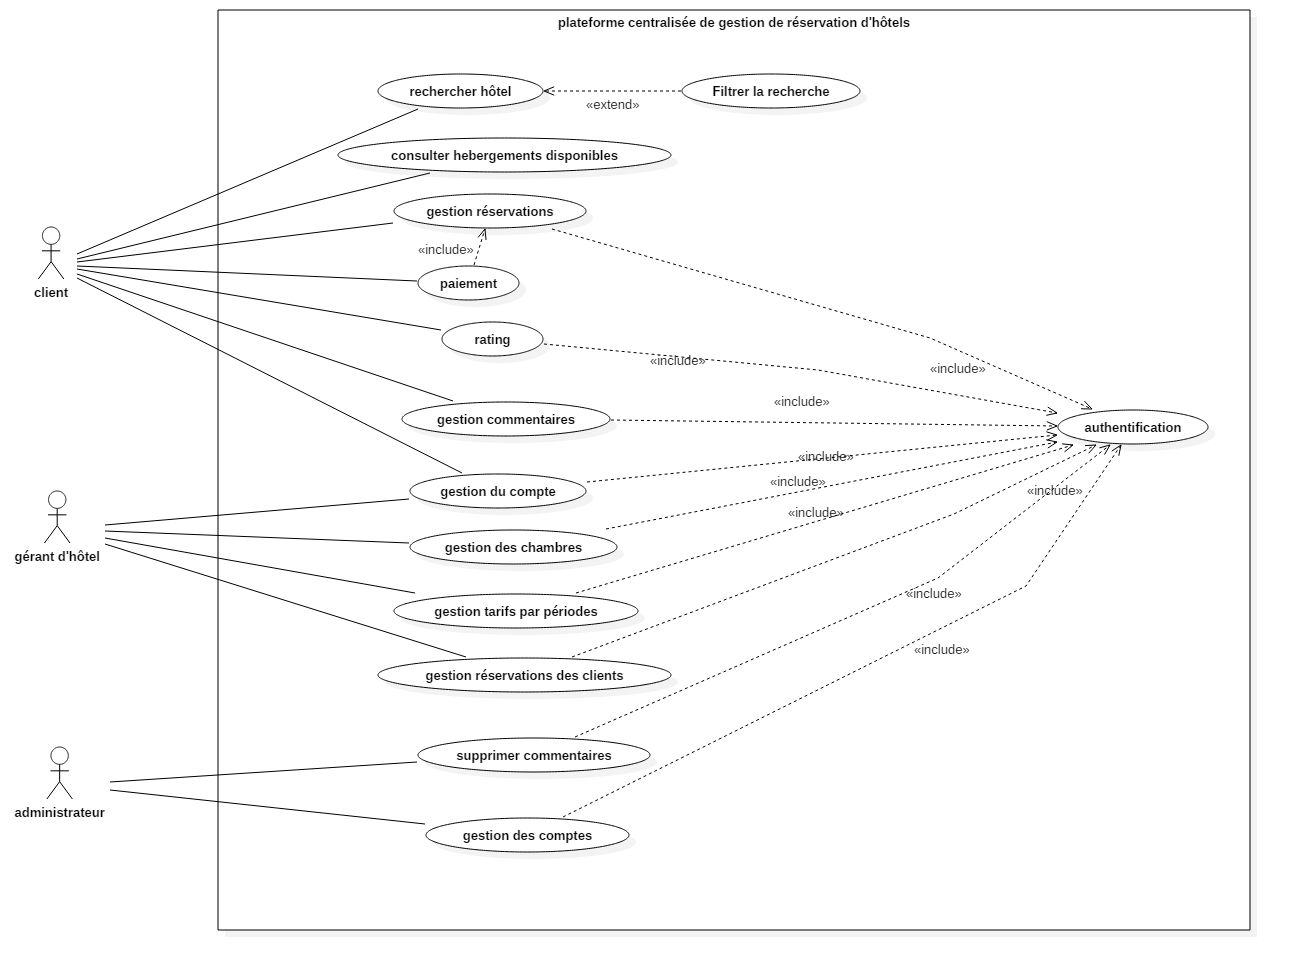
\includegraphics[scale=0.35]{./graphics/diag_usecase.png}
				\caption{Diagramme de cas d'utilisation}
			\end{figure}
			\newpage
		
			

		%================vue dynamique====================
	
		\newpage
		\section{Conception}
			\subsection{Diagramme de séquence:} 
Ces diagrammes sont la représentation graphique des interactions entre les acteurs et le
système selon un ordre chronologique. Ces interactions sont ainsi montrées dans le cadre d'un
scénario d'un diagramme de cas d'utilisation et ils ont pour but de décrire comment se déroule les
actions entre les acteurs ou objets.
			
			\subsection{scénario de réservation d'hôtel}
			\vspace{1cm}
			\begin{figure}[!hbtp]
				\centering
				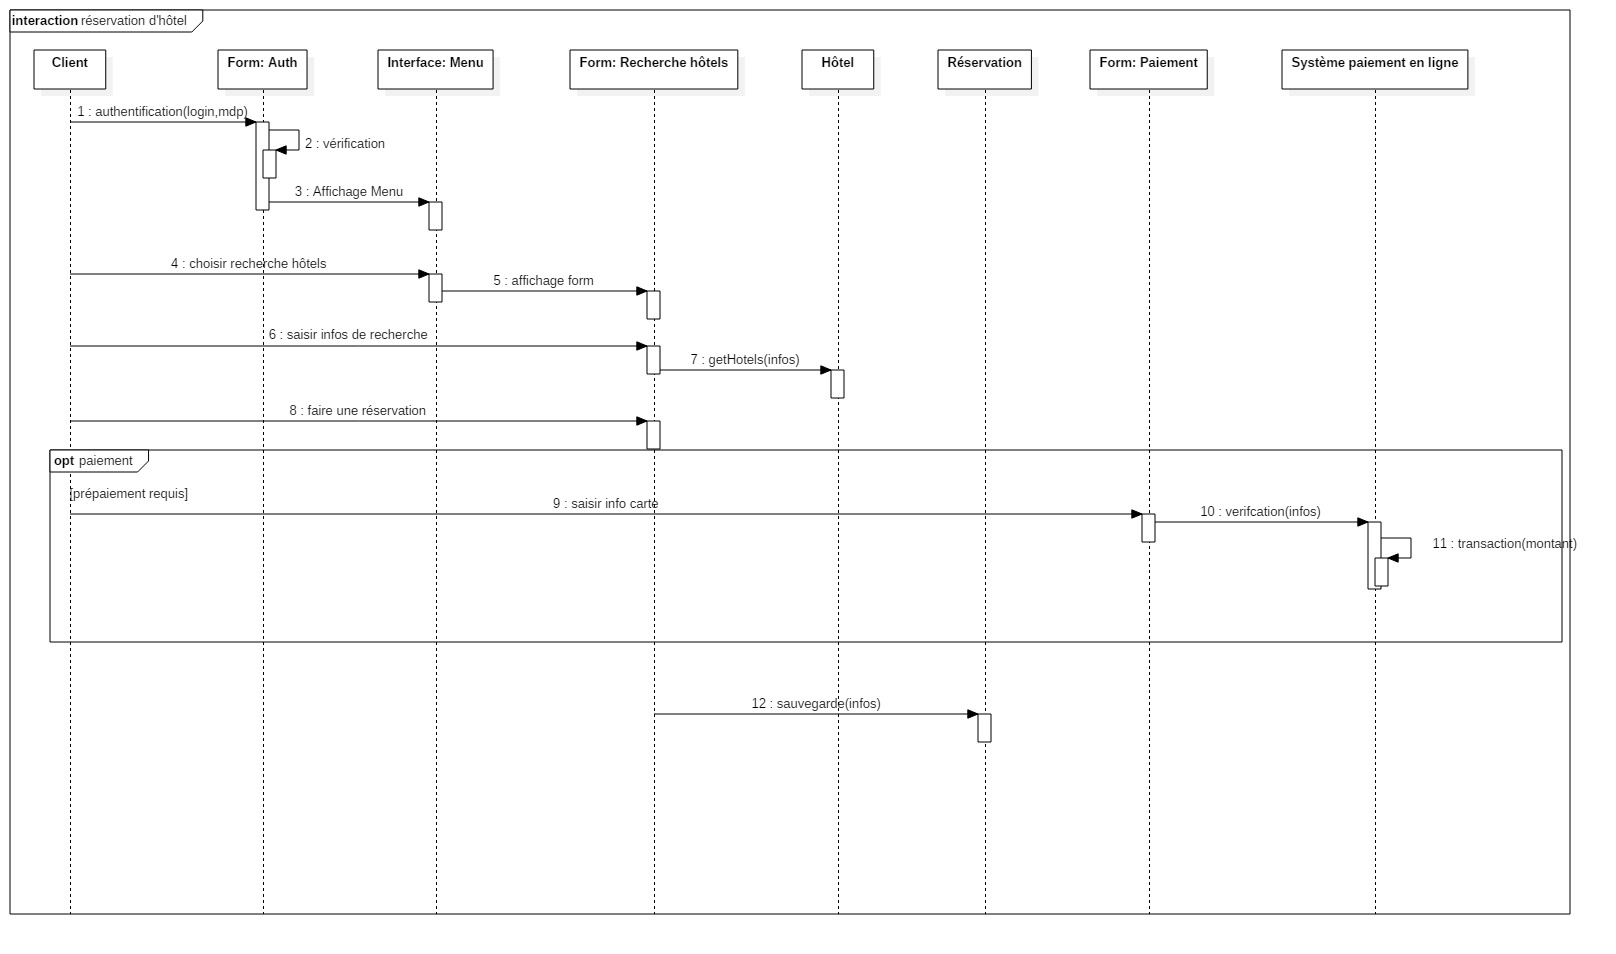
\includegraphics[scale=0.31]{./graphics/scenario_reservation.jpg}
				\caption{Scénarion de réservation d'hôtel}
			\end{figure}

			\newpage
			
			\subsection{scénario de paiement en ligne}
			\vspace{1cm}
			\begin{figure}[!hbtp]
				\centering
				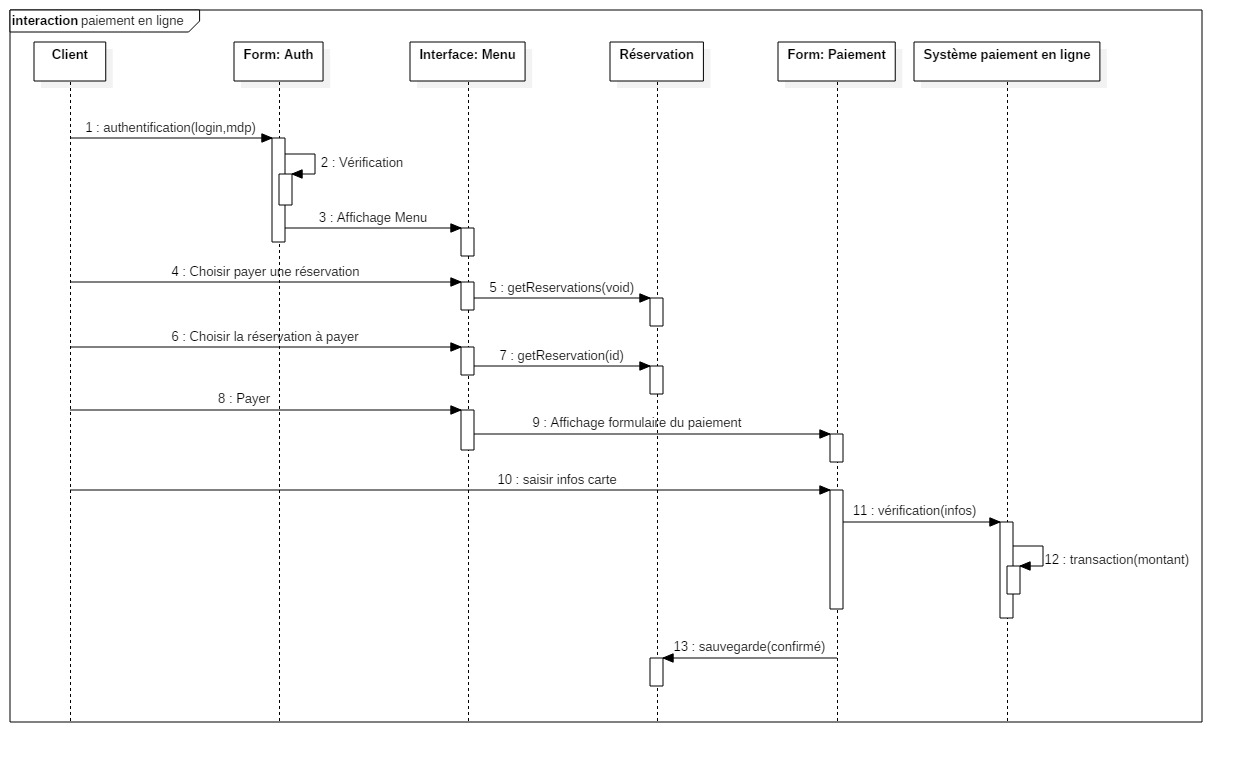
\includegraphics[scale=0.35]{./graphics/paiement.jpg}
				\caption{Scénarion de paiement en ligne}
			\end{figure}

			\newpage
		

		%===================diag de classe===========================
			\subsection{Diagramme de classe}
			Le diagramme de classe est un élément important dans une démarche de conception orientée
			objet. Il représente les différentes entités (les classes d'objet) intervenant dans le système. Après
			l’analyse des différents diagrammes de séquences élaborés, nous avons construit progressivement le
			diagramme de classes.
			\vspace{2cm}
			\begin{figure}[!hbtp]
				\centering
				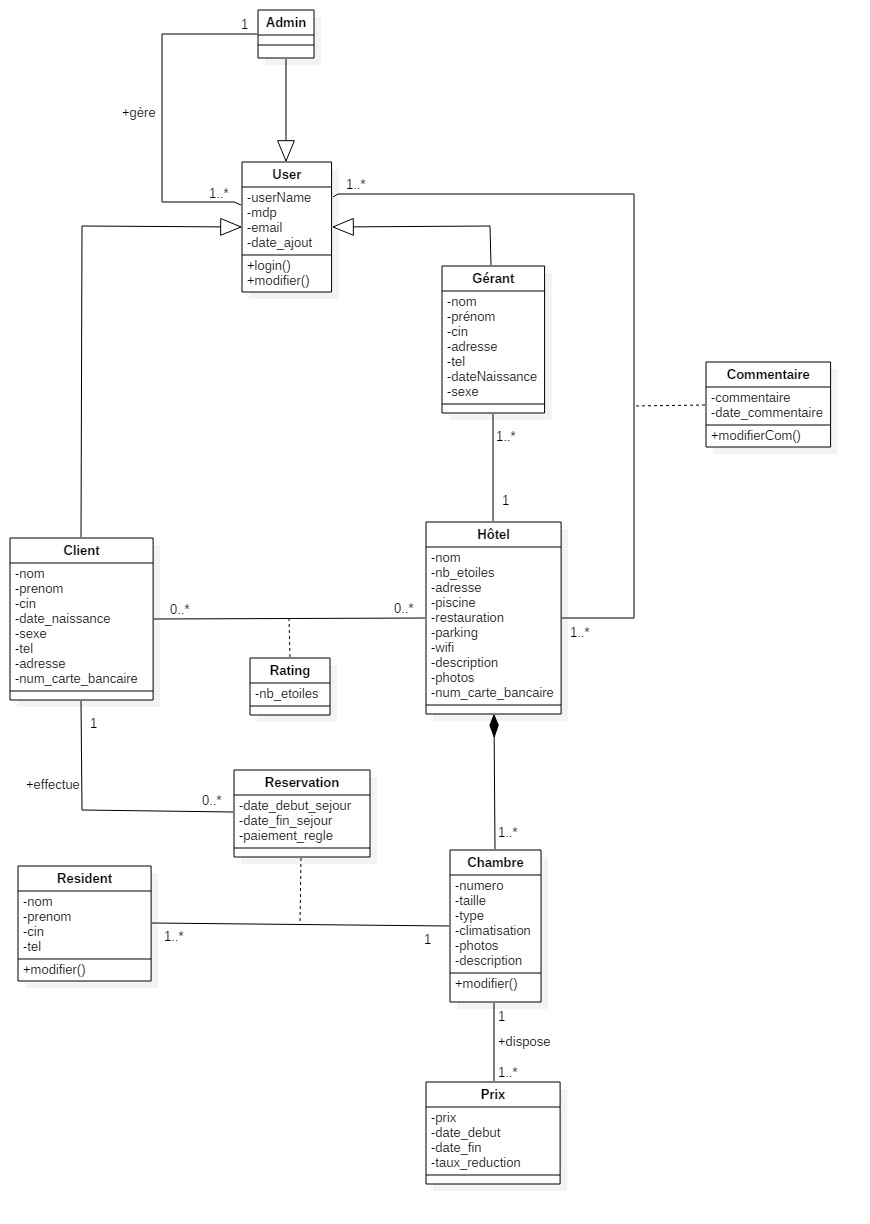
\includegraphics[scale=0.34]{./graphics/diag_classe.png}
				\caption{Diagramme de classe}
			\end{figure}
			\newpage
		
		%===========conclusion===========
		\section{Conclusion}
Dans ce chapitre, j'ai présenté l'étude analytique conceptuelle du système. La vue fonctionnelle a été illustrée par un diagramme de cas d’utilisation, la vue dynamique par un diagramme de séquence qui ma permis d'avoir une vue générale sur le déroulement des cas d'utilisation et leurs exécutions. Enfin, le diagramme de classe qui m'a permis de définir la structure du système et de dégager les différentes classes le composant.\\
Dans le chapitre suivant, on définit les zones et les composants de l’interface de l'application à travers quelques maquettes.	
%===========================================fin chapitre analyse et conception =========================




	


%==========================================maquettes===============================
	\chapter{Maquettes}
Le mock-up, ou dit autrement la maquette fonctionnelle, montre la partie visuelle
du projet. Il s’agit d’une représentation statique du contenu, de la structure
et des fonctionnalités de l’application.\\
Enfin, le prototype est une maquette interactive. En plus de la partie visuelle,
il montre le fonctionnement de l’application. Le prototype est extrêmement utile
pour tester la convivialité du projet.\\
	
	
	\section{Authentification}
	\begin{figure}[!hbtp]
		\centering
		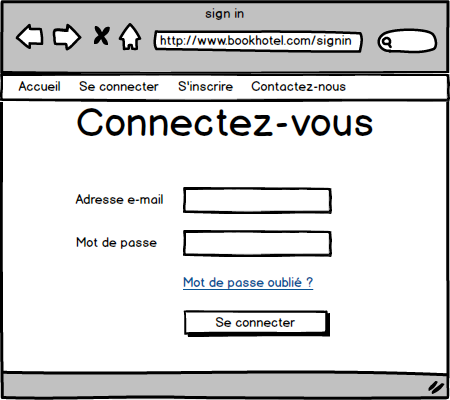
\includegraphics[scale=0.5]{./graphics/1.png}
		\caption{Maquette authentification}
	\end{figure}
	
	\newpage 

	\section{Création de compte}
	\begin{figure}[!hbtp]
		\centering
		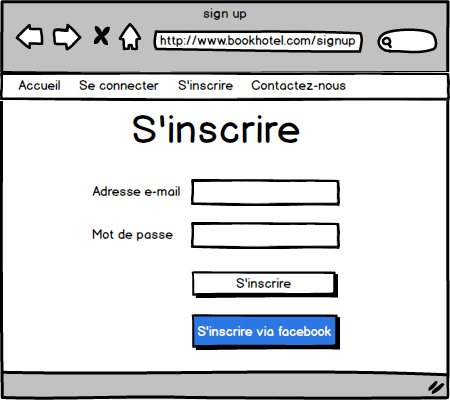
\includegraphics[scale=0.5]{./graphics/2.png}
		\caption{Maquette création de compte}
	\end{figure}

		
	
	\section{Paramètre du compte}
	\begin{figure}[!hbtp]
		\centering
		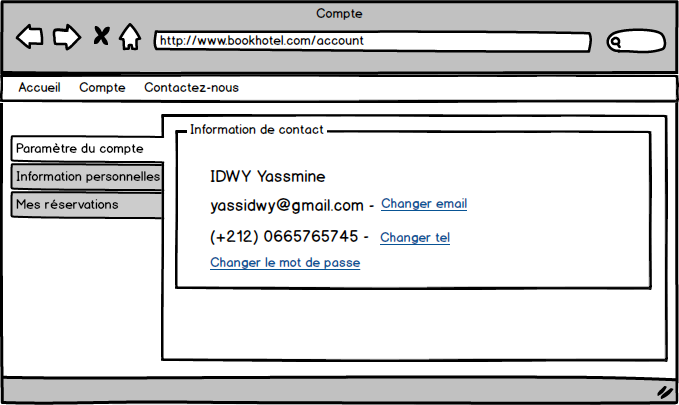
\includegraphics[scale=0.5]{./graphics/6.png}
		\caption{Maquette paramètre du compte}
	\end{figure}
	
	\newpage
	\section{Informations personnelles}
	\vspace{2cm}
	\begin{figure}[!hbtp]
		\centering
		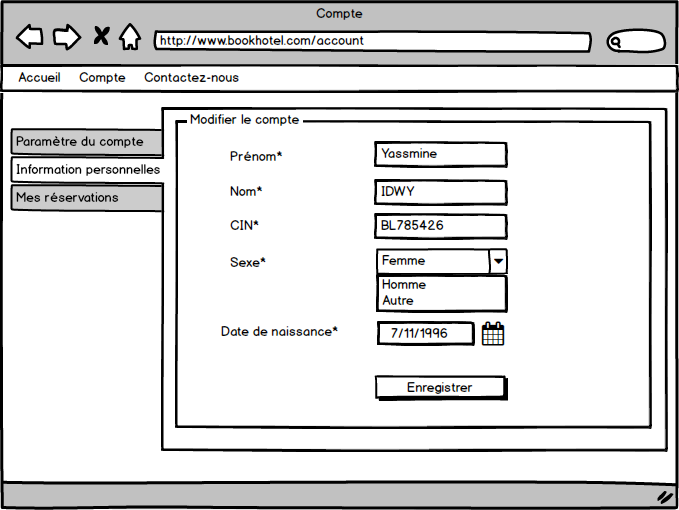
\includegraphics[scale=0.5]{./graphics/7.png}
		\caption{Maquette informations personnelles}
	\end{figure}

	\newpage
	\section{Mes réservations}
	\begin{figure}[!hbtp]
		\centering
		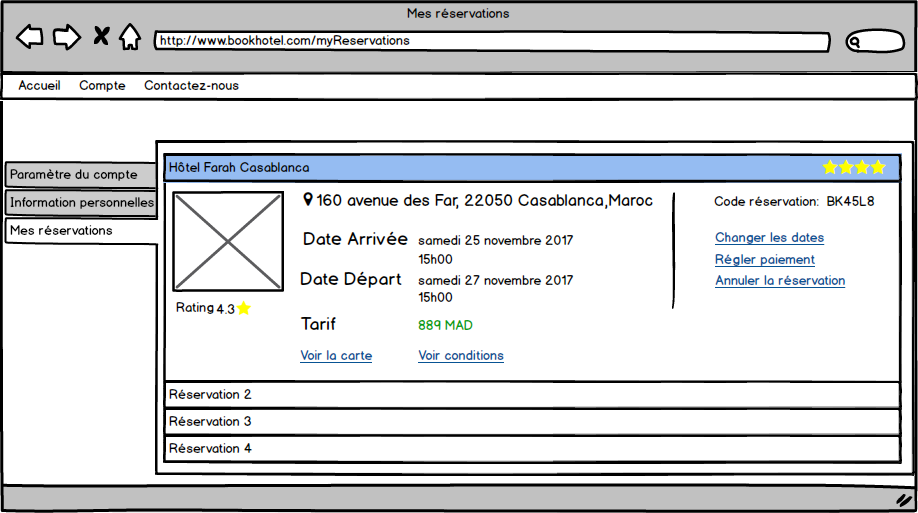
\includegraphics[scale=0.4]{./graphics/4.png}
		\caption{Maquette mes réservations}
	\end{figure}
	
	
	\section{Recherche d'hôtel}
	\begin{figure}[!hbtp]
		\centering
		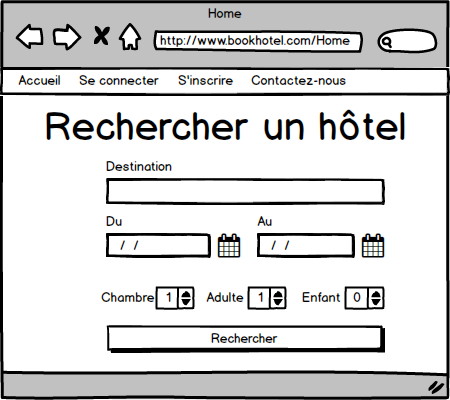
\includegraphics[scale=0.5]{./graphics/3.png}
		\caption{Maquette recherche d'hôtel}
	\end{figure}
	
	
	\newpage
	\section{Hôtels disponibles}
	\vspace{2cm}
	\begin{figure}[!hbtp]
		\centering
		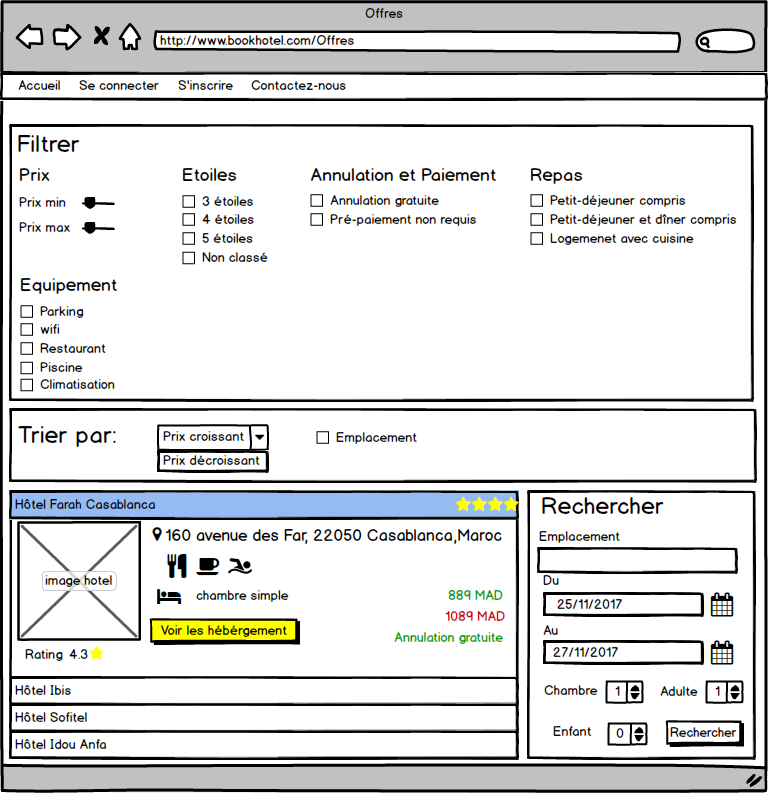
\includegraphics[scale=0.5]{./graphics/5.png}
		\caption{Maquette hôtels disponibles}
	\end{figure}

	\newpage
	\section{Hébérgements}
	\begin{figure}[!hbtp]
		\centering
		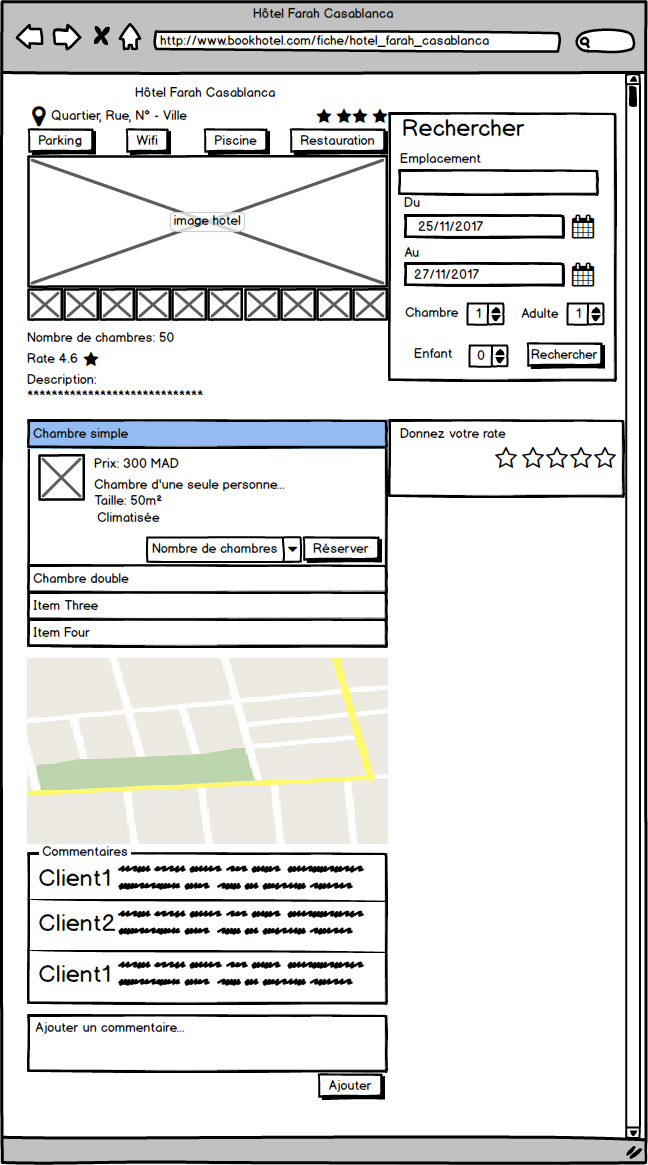
\includegraphics[scale=0.4]{./graphics/9.png}
		\caption{Maquette hébérgements}
	\end{figure}
	
	\newpage
	\section{Réservation}
	\begin{figure}[!hbtp]
		\centering
		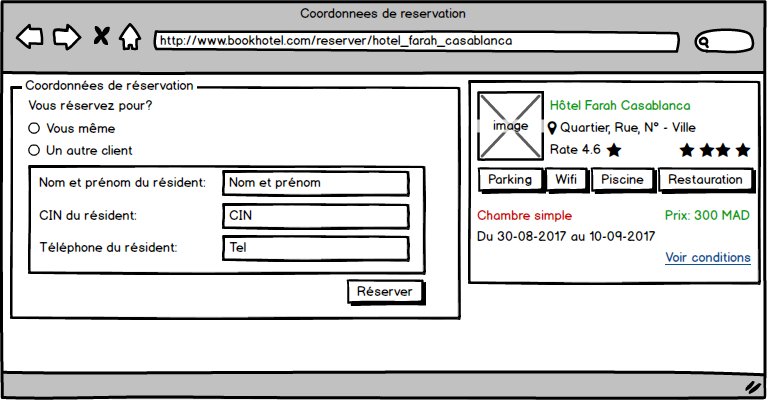
\includegraphics[scale=0.5]{./graphics/10.png}
		\caption{Maquette réservation}
	\end{figure}
	
	\section{Paiement}
	\begin{figure}[!hbtp]
		\centering
		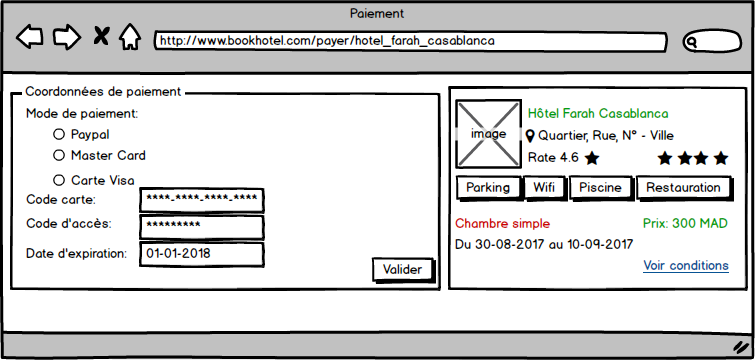
\includegraphics[scale=0.5]{./graphics/11.png}
		\caption{Maquette paiement}
	\end{figure}

	\newpage
	\section{Ajouter un hôtel}
	\begin{figure}[!hbtp]
		\centering
		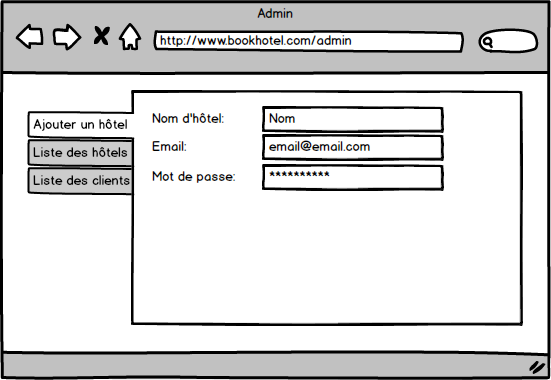
\includegraphics[scale=0.5]{./graphics/12.png}
		\caption{Maquette ajouter un hôtel}
	\end{figure}
	
	\section{Liste des hôtels}
	\begin{figure}[!hbtp]
		\centering
		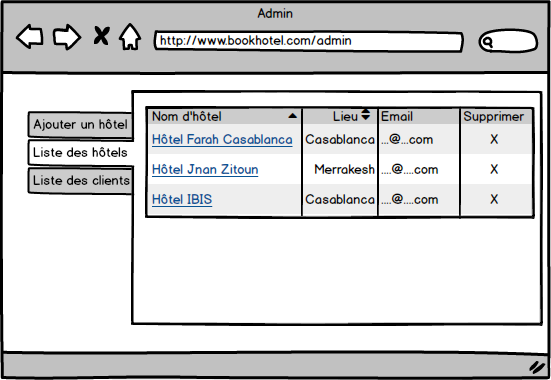
\includegraphics[scale=0.5]{./graphics/8.png}
		\caption{Maquette liste des hôtels}
	\end{figure}


	\section{Liste des clients}
	\vspace{2cm}
	\begin{figure}[!hbtp]
		\centering
		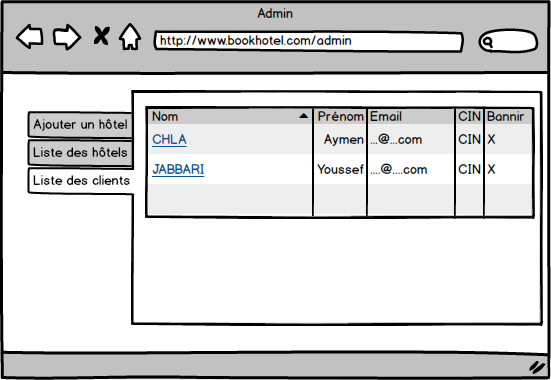
\includegraphics[scale=0.5]{./graphics/13.png}
		\caption{Maquette liste des clients}
	\end{figure}

%========================================fin maquette=============================










%=========================chapitre 3===========================
		\chapter{Conception technique}
		

		%=========intro==============
		\section{Introduction}
Il s’agit dans ce chapitre d’identifier les différentes caractéristiques de l’environnement logiciel ainsi que les technologies qui nous ont servi à l’implémentation de notre application.		
		
		\section{Architecture technique}
		Dans le but de réaliser un système puissant, évolutif et modulaire nous allons adopter une
architecture en couches, qui est la conséquence inéluctable d’une approche qui s’appuie sur la
réalisation de composants réutilisables, et qui nous garantit le maximum de découplage entre les
couches logicielles mises en œuvre.
		
		\begin{figure}[!hbtp]
			\centering
			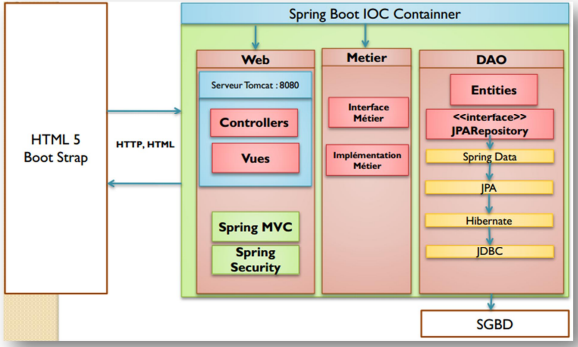
\includegraphics[scale=0.5]{./graphics/architecture_tech.png}
			\caption{Architecture technique}
		\end{figure}
		\newpage
		
	\section{Frameworks}
		\subsection{Spring}
		\begin{wrapfigure} {r}{3cm}
		
\includegraphics[scale=0.25]{./graphics/spring.png}
		\end{wrapfigure}
		En informatique, Spring est un framework libre pour construire et définir l'infrastructure d'une application java, dont il facilite le développement et les tests.\\
Spring est modulaire, permettant de choisir les modules appropriés à votre application, sans être obligé d'utiliser le reste.\\
Spring fournit plus de 20 modules qui peuvent être utilisé dans les applications, pour notre cas nous avons opté pour : \\
		\begin{itemize}
				\item \textbf{Spring Core:} Un conteneur qui implémente le motif de conception IoC (Inversion of Control). Ce conteneur prend en charge la création, la gestion du cycle de vie et les dépendances des objets qu'il gère.
				\item \textbf{Spring MVC:} Une implémentation innovante du patron MVC qui profite des avantages de l’injection de dépendances et qui, depuis la version 2.5, offre une intéressante flexibilité grâce aux annotations
Java 5. Ce module permet dès lors de s’abstraire de l’API Servlet de Java EE.
				\item \textbf{Spring Security :} Un conteneur qui gère l'authentification et le contrôle d'accès.
				\item \textbf{Spring Boot:} un micro framework qui a notamment pour but de faciliter la configuration d'un projet Spring et de réduire le temps alloué au démarrage d'un projet.	
				\end{itemize}
		
		\subsection{Hibernate}
		\begin{wrapfigure} {r}{3cm}
		
\includegraphics[scale=0.25]{./graphics/hibernate.jpg}
		\end{wrapfigure}
		Hibernate est un framework open source gérant la persistance des objets en base de données relationnelle.\\
Hibernate est adaptable en termes d'architecture, il peut donc être utilisé aussi bien dans un développement client lourd, que dans un environnement web léger de type Apache Tomcat ou dans un environnement Java EE complet: WebSphere, JBoss Application Server et Oracle WebLogic Server.\\
		\newpage
		\subsection{Bootstrap}
		\begin{wrapfigure} {r}{3cm}
		
\includegraphics[scale=0.25]{./graphics/bootstrap.png}
		\end{wrapfigure}
		Bootstrap fournit une feuille de style CSS qui contient des définitions de base pour tous les composants HTML, ce qui permet de disposer d'une apparence uniforme pour les textes, tableaux et les éléments de formulaires.\\

		
	\section{outils}
		\subsection{Maven}
		\begin{wrapfigure} {r}{3cm}
		
\includegraphics[scale=0.3]{./graphics/maven.png}
		\end{wrapfigure}
		Maven est un outil de construction de projets (build) open source développé par la fondation Apache, initialement pour les besoins du projet Jakarta Turbine. Il permet de faciliter et d'automatiser certaines tâches de la gestion d'un projet Java.\\

		\subsection{MySQL}
		\begin{wrapfigure} {r}{3cm}
		
\includegraphics[scale=0.3]{./graphics/mysql.png}
		\end{wrapfigure}
		MySQL est un système de gestion de bases de données relationnelles (SGBDR). Il est distribué sous une double licence GPL et propriétaire. Il fait partie des logiciels de gestion de base de données les plus utilisés au monde3, autant par le grand public (applications web principalement) que par des professionnels, en concurrence avec Oracle, Informix et Microsoft SQL Server.\\

		\subsection{Trello}
		\begin{wrapfigure} {r}{3cm}
		
\includegraphics[scale=0.25]{./graphics/trello.png}
		\end{wrapfigure}
		Trello est un outil de gestion de projet en ligne, lancé en septembre 2011, et inspiré par la méthode Kanban de Toyota. Il est basé sur une organisation des projets en planches listant des cartes, chacune représentant des tâches. Les cartes sont assignables à des utilisateurs et sont mobiles d'une planche à l'autre, traduisant leur avancement.\\
		
		\newpage
		\subsection{\LaTeX}
		\begin{wrapfigure} {r}{3cm}
		
\includegraphics[scale=0.05]{./graphics/latex.png}
		\end{wrapfigure}
\LaTeX est un langage et un système de composition de documents
créé par Leslie Lamport en 1983. C’est un ensemble de
macro-commandes basées sur le langage TEX – developpé par
Donald Knuth.Il permettant de créer des documents écrits de grande qualité : principalement livres et articles, mais aussi, courriers, présentations projetées.\\
			
		\subsection{Git et Github}
		\begin{wrapfigure} {r}{3cm}
		
\includegraphics[scale=0.25]{./graphics/gitgithub.jpg}
		\end{wrapfigure}
		Git est un système de contrôle de version (VCS) pour suivre les changements dans les fichiers et coordonner le travail sur ces fichiers entre plusieurs personnes. Il est principalement utilisé pour le développement de logiciels, mais il peut être utilisé pour garder une trace des changements dans les fichiers.\\
Github est un service web d'hébergement et de gestion de développement logiciel utilisant les logiciels de gestion de versions Git.\\

		
		\subsection{Google Map Api}
		\begin{wrapfigure} {r}{3cm}
		
\includegraphics[scale=0.15]{./graphics/google.png}
		\end{wrapfigure}
		Google Maps est un service gratuit de cartographie en ligne. Le service a été créé par Google.\\


		\section{Conclusion}
Au cours de ce chapitre, J'ai présenté l’environnement de développement et les différents outils utilisés pour la mise en place de l’application.\\
Dans le chapitre suivant, je détaille quelques aspects de la réalisation.

%===============================fin chapitre conception  technique===================












%================================chapitre Réalisation==============================
	\chapter{Réalisation}

	\section{Introduction}
Nous faisons preuve, à travers ce chapitre, des différentes interfaces développées par rapport
à ce projet, et nous expliquons le rôle de chacune.
Les figures ci-dessous représentent quelques captures d’écran de pages de notres application. Les pages qui suivent l’authentification contiennent tous un menu, qui va nous permettre de naviguer dans les différentes pages de l'application.\\


	\section{Partie client}
Dans cette partie nous alons décrire la réalisation sous forme d’un scénario de réservation d'hôtel.
	\newpage
	\subsection{Page d'accueil}
	\vspace{2cm}
	\begin{figure}[!hbtp]
		\centering
		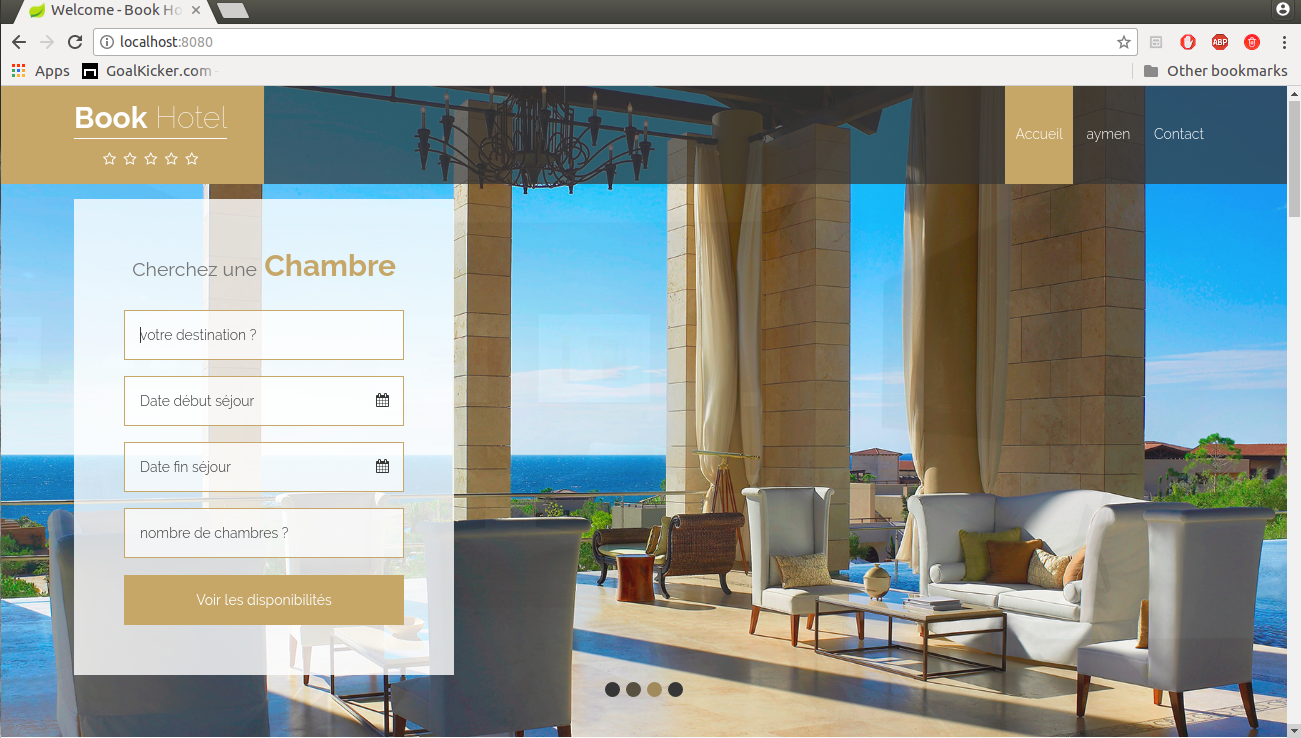
\includegraphics[scale=0.3]{./graphics/home.png}
		\caption{Page d'accueil}
		\end{figure}
		\newpage

	\subsection{Hôtels disponibles}
	\vspace{2cm}
	\begin{figure}[!hbtp]
		\centering
		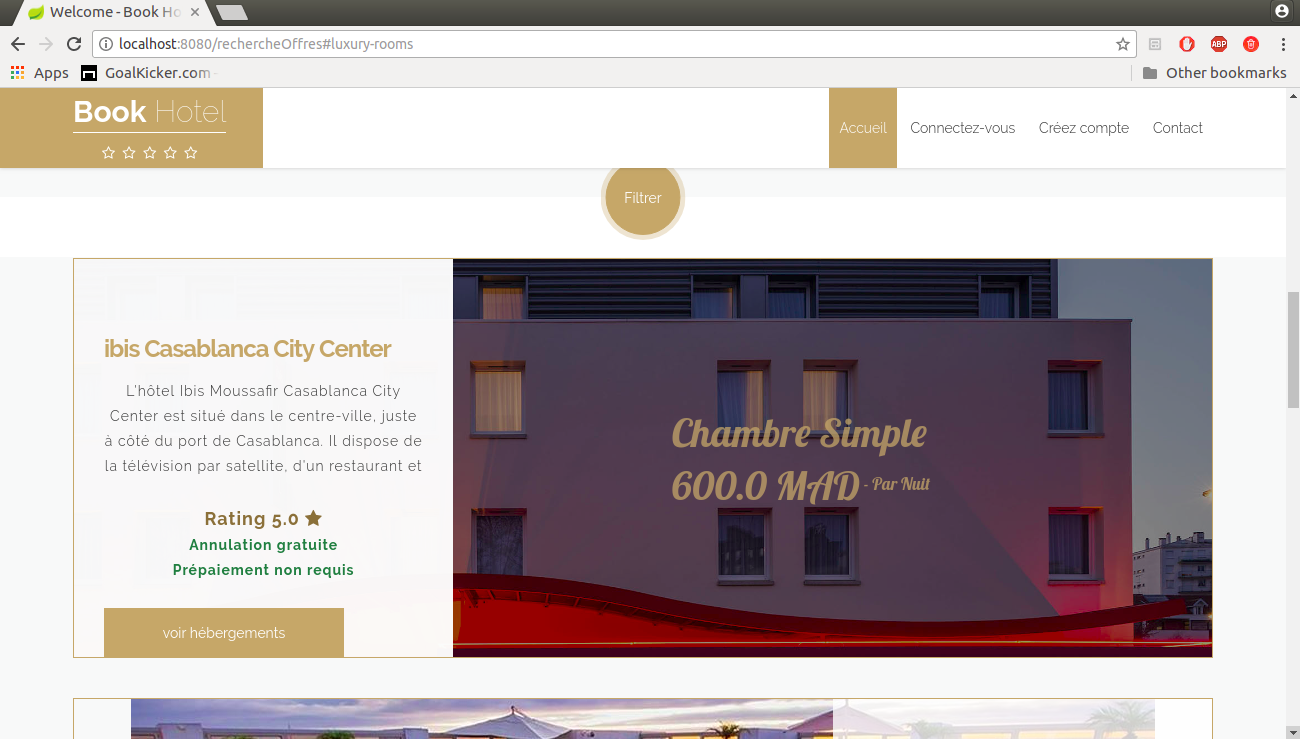
\includegraphics[scale=0.3]{./graphics/offres.png}
		\caption{Hôtels disponibles}
		\end{figure}
		\newpage
	
	\subsection{Hébergements disponibles dans un hôtel}
Cette page est divisées en quatres parties:
	\begin{itemize}
	 		\item Rating et information de l'hôtel.
			\item Chambres disponibles.
			\item Une Map pour localiser l'hôtel.
			\item Partage d'avis (Commentaires).
		\end{itemize}
	
	\subsubsection{Rating et informations de l'hôtel}
	La première partie de cette page affiche les informations concernant l'hôtel, elle donne aussi la possiblité de faire du \guillemotleft Rating \guillemotright.\\
	Ici on remarque que le rate est de 3.5/5 pour un rating de 2 clients.\\
	Une seule personne à voter pour 5 étoiles.\\
	Une seule personne à voter pour 2 étoiles
	\vspace{2cm}
	\begin{figure}[!hbtp]
		\centering
		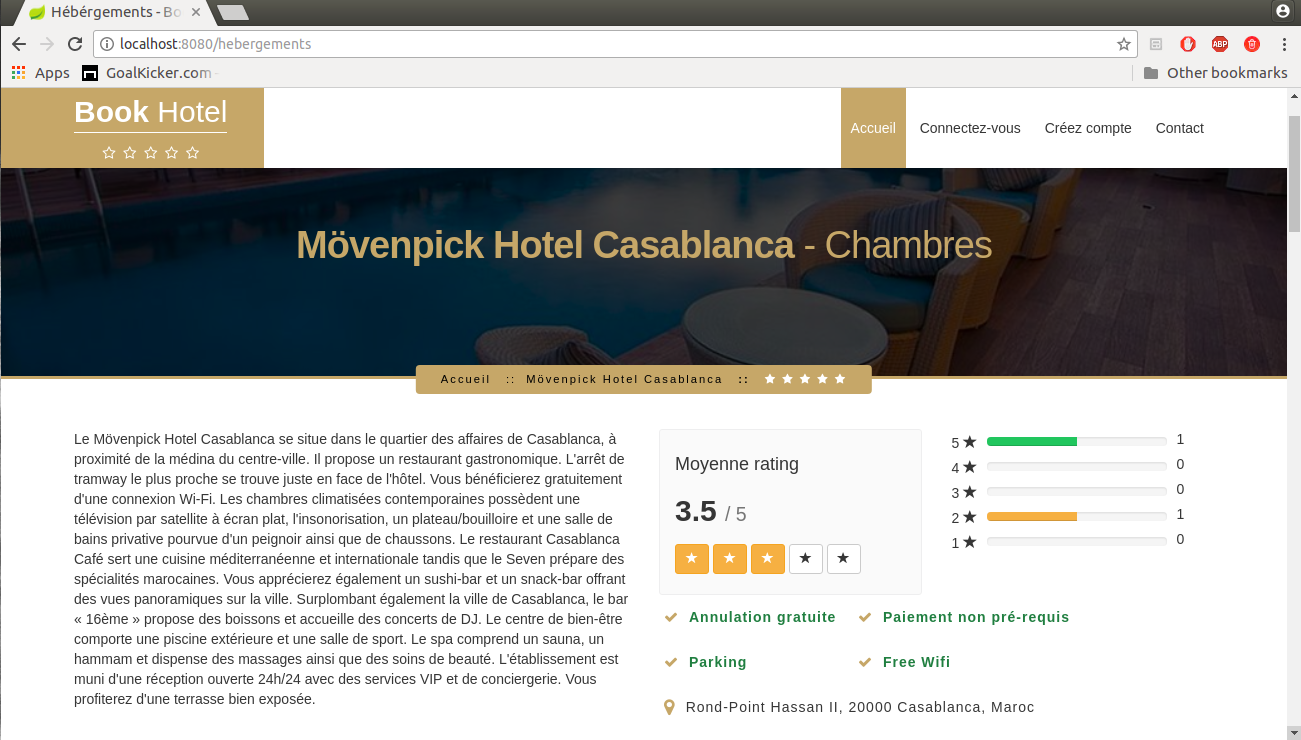
\includegraphics[scale=0.3]{./graphics/rating.png}
		\caption{Rating et informations de l'hôtel}
		\end{figure}
		\newpage

	\subsubsection{chambres disponibles}
	La deuxième partie de cette page affiche les chambres disponibles dans l'hôtel, on peut choisir le nombre de chambres souhaitées pour passer ensuite à la réservation.\\
	\vspace{2cm}
	\begin{figure}[!hbtp]
		\centering
		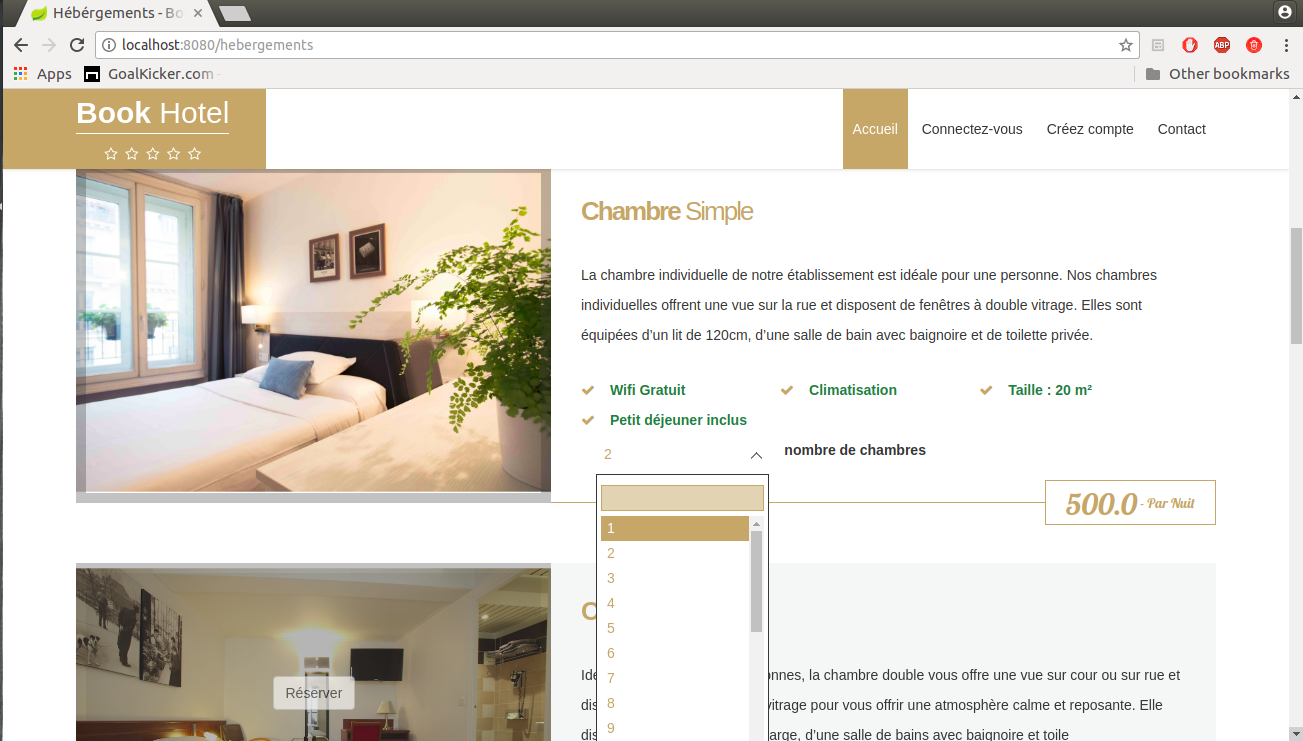
\includegraphics[scale=0.3]{./graphics/hebergement.png}
		\caption{chambres disponibles}
		\end{figure}
		\newpage

	\subsubsection{Localisation de l'hôtel}
	La troisième partie de cette page montre la position géographique de l'hôtel.\\
	\vspace{2cm}
	\begin{figure}[!hbtp]
		\centering
		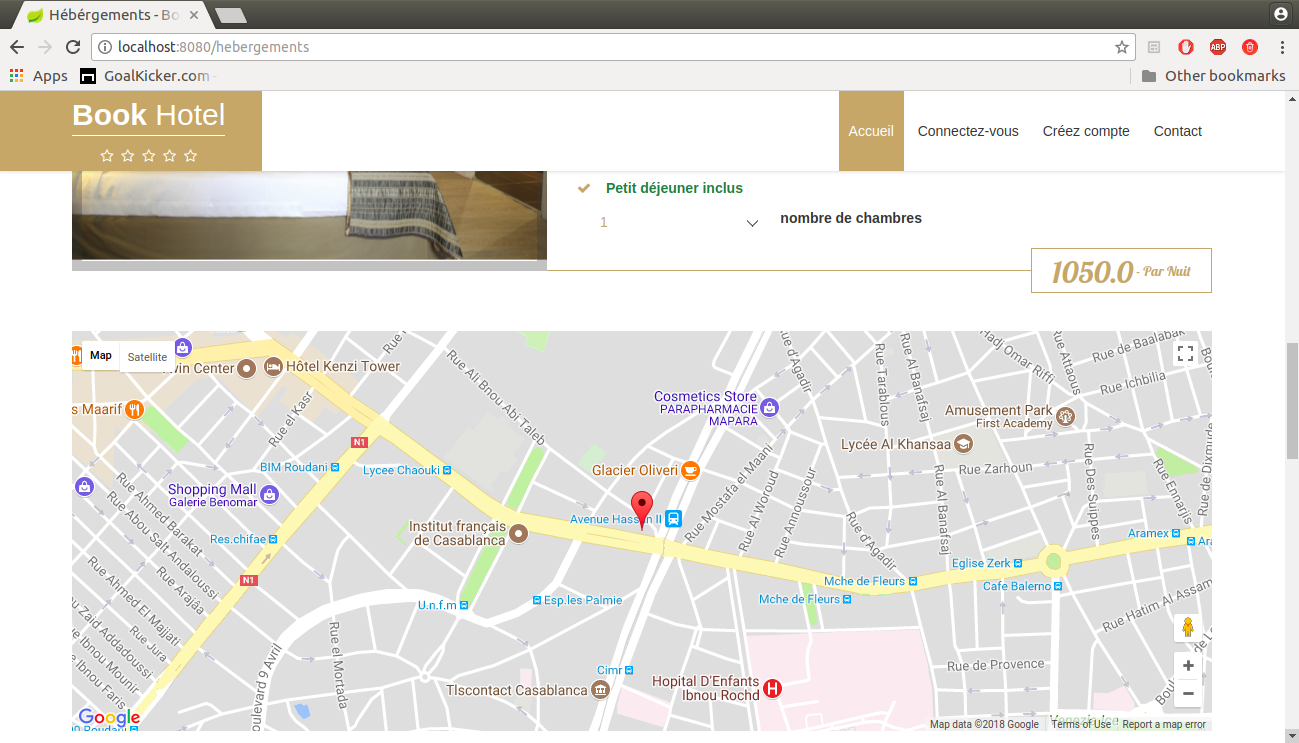
\includegraphics[scale=0.3]{./graphics/map.png}
		\caption{Localisation de l'hôtel}
		\end{figure}
		\newpage

	\subsubsection{Partage d'avis}
	La quatrième partie de cette page affiche les avis concernants l'hôtel. On peut commenter et supprimer nos propres commentaires\\
	\vspace{2cm}
	\begin{figure}[!hbtp]
		\centering
		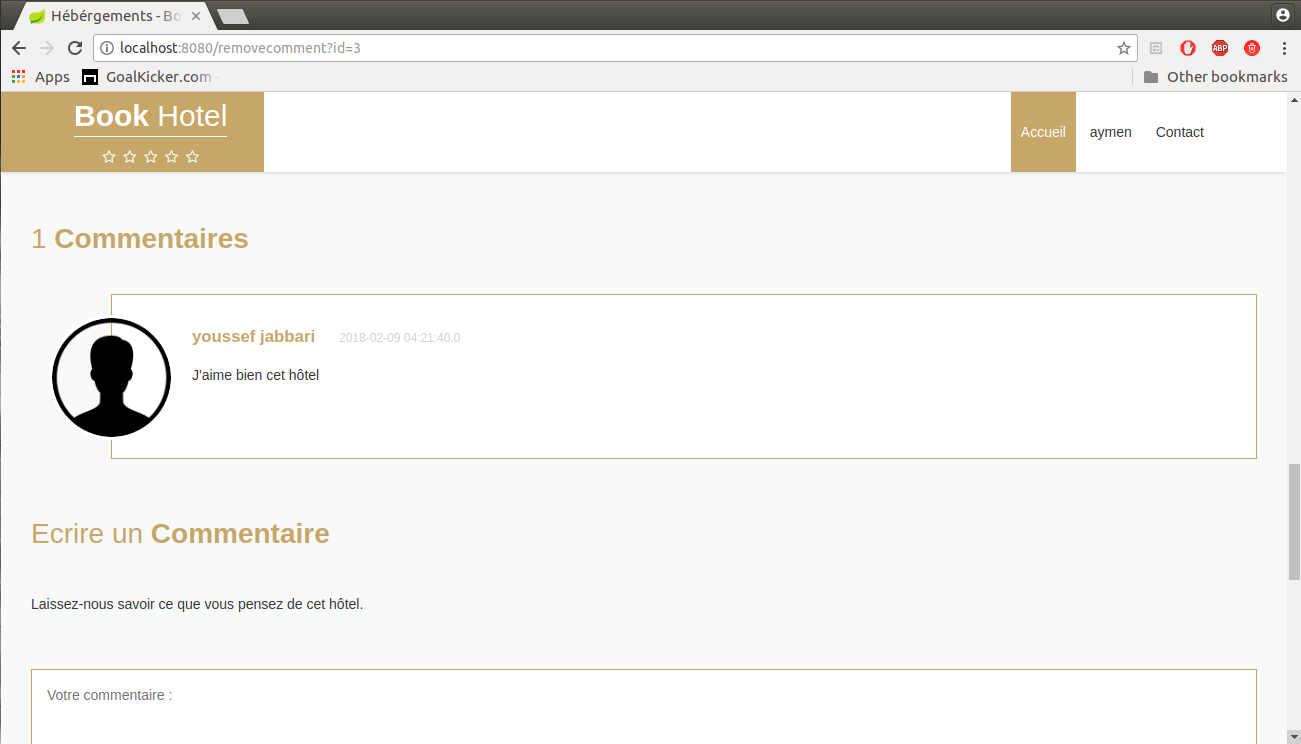
\includegraphics[scale=0.3]{./graphics/comment.png}
		\caption{Partage d'avis}
		\end{figure}
		\newpage



	\subsection{Authentification et création de compte}
Pour effectuer une réservation il est primordiale de s'authentifier ou créer un compte.
	\vspace{2cm}
	\begin{figure}[!hbtp]
		\centering
		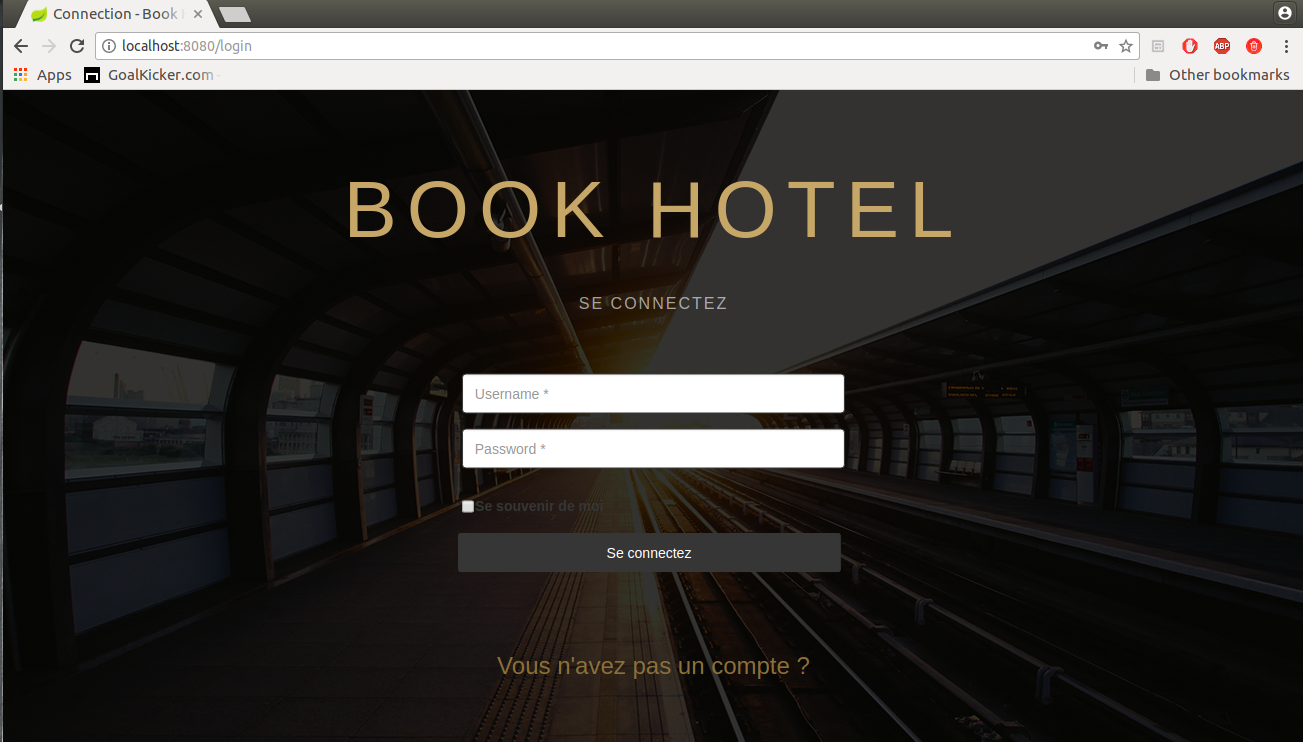
\includegraphics[scale=0.2]{./graphics/login.png}
		\caption{Authentification}
		\end{figure}
	\begin{figure}[!hbtp]
		\centering
		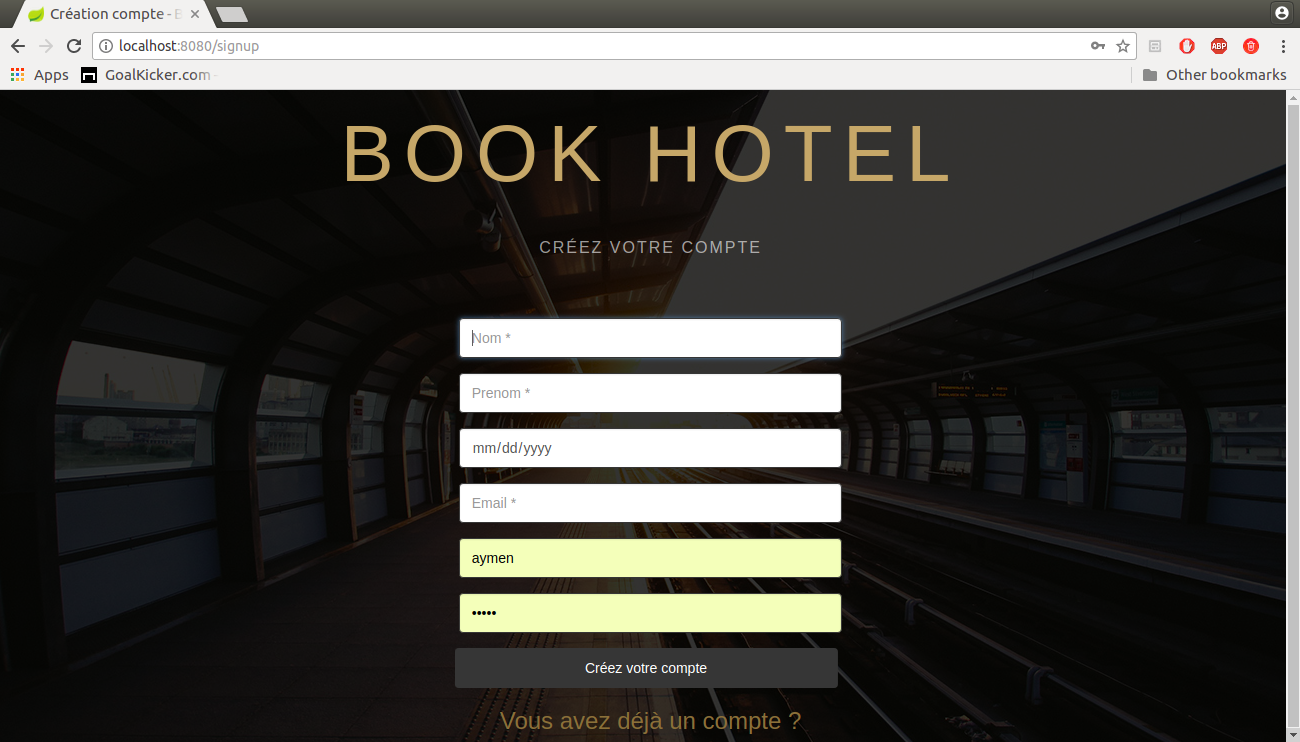
\includegraphics[scale=0.2]{./graphics/signup.png}
		\caption{création de compte}
		\end{figure}
		\newpage

	\subsection{Réservation}
Pour réserver il faut saisir les informations du résident de chaque chambre.\\
Si le résident d'une chambre est le client authetifié on peut passer directement au paiement.
	\vspace{2cm}
	\begin{figure}[!hbtp]
		\centering
		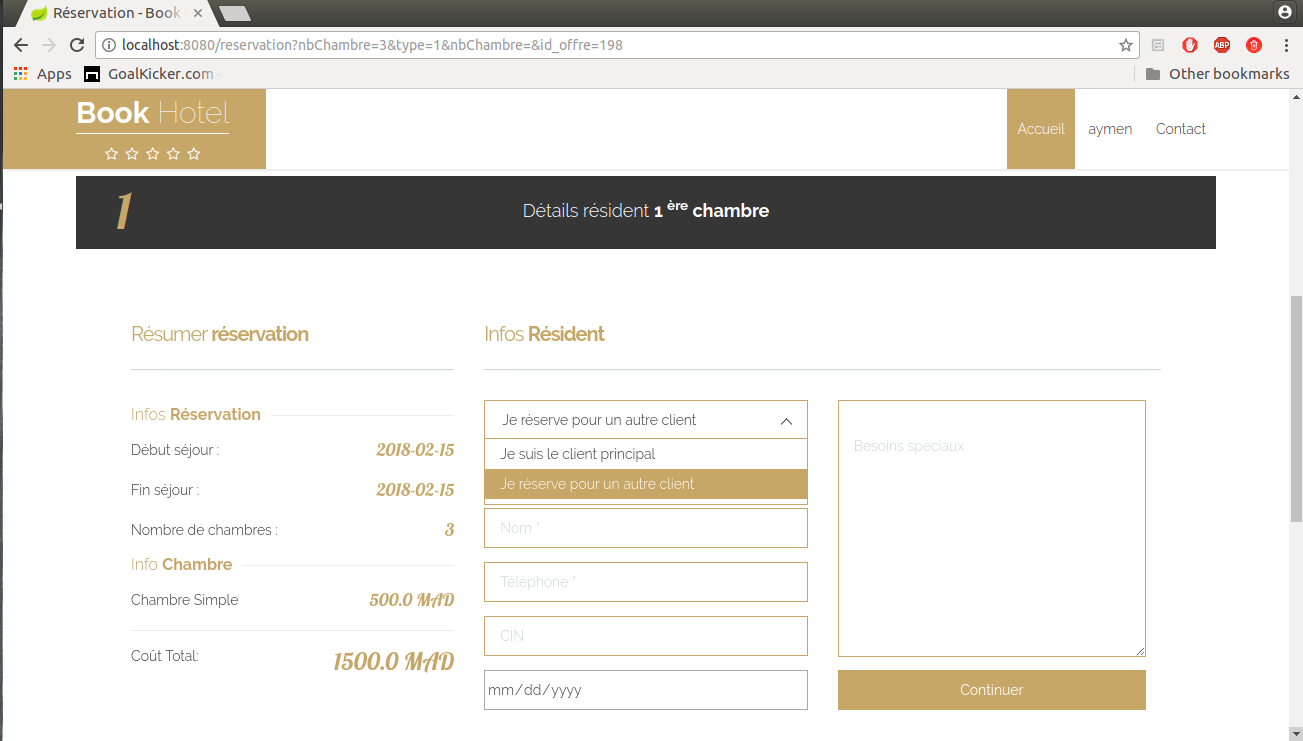
\includegraphics[scale=0.3]{./graphics/reservation.png}
		\caption{Réservation}
		\end{figure}
		\newpage
	
	\subsubsection{Paiement}
Cette page affiche un résumer sur la réservation, et permet de confirmer la réservation par le paiement.\\
Si le paiement n'est pas pré-requis un bouton s'affiche en bas du formulaire pour sauter la phase de paiement.\\
	\vspace{2cm}
	\begin{figure}[!hbtp]
		\centering
		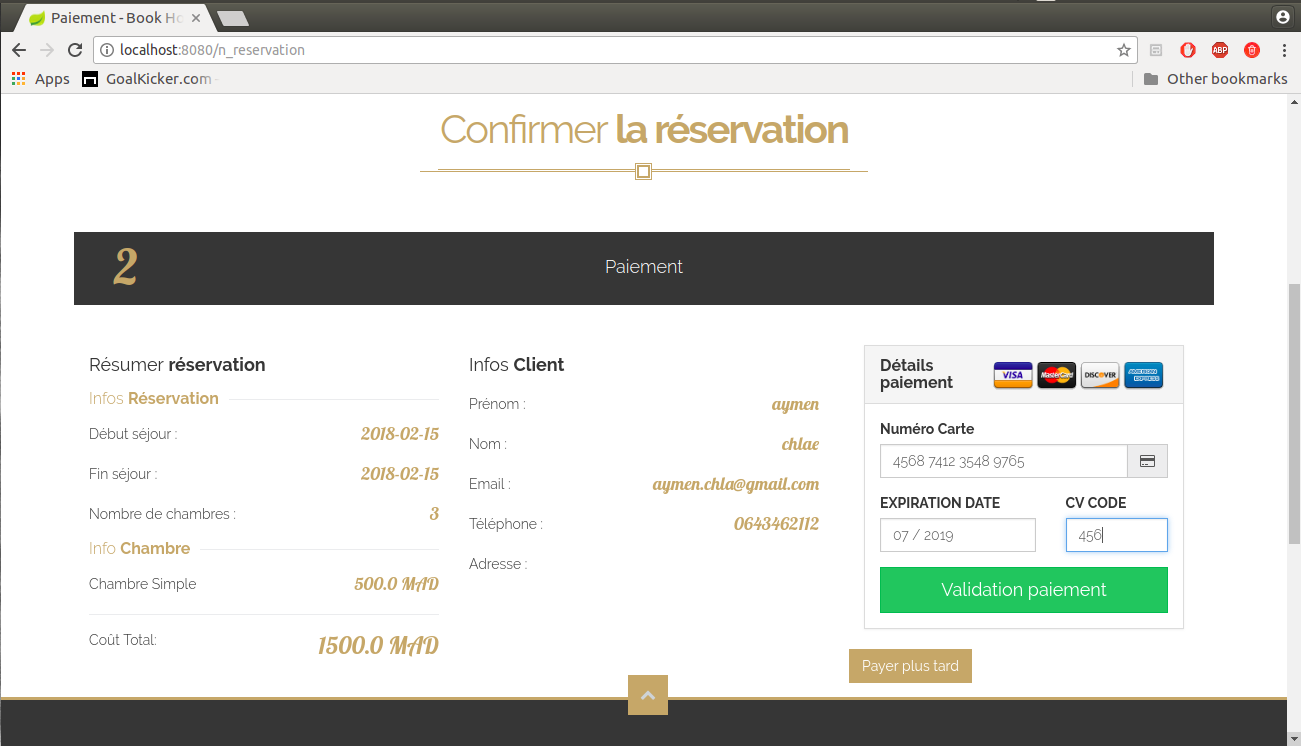
\includegraphics[scale=0.3]{./graphics/paiement.png}
		\caption{Paiement}
		\end{figure}
		\newpage

	\subsubsection{Mes réservations}
On peut consulter, regler le paiement et annuler les réservations.\\
	\vspace{2cm}
	\begin{figure}[!hbtp]
		\centering
		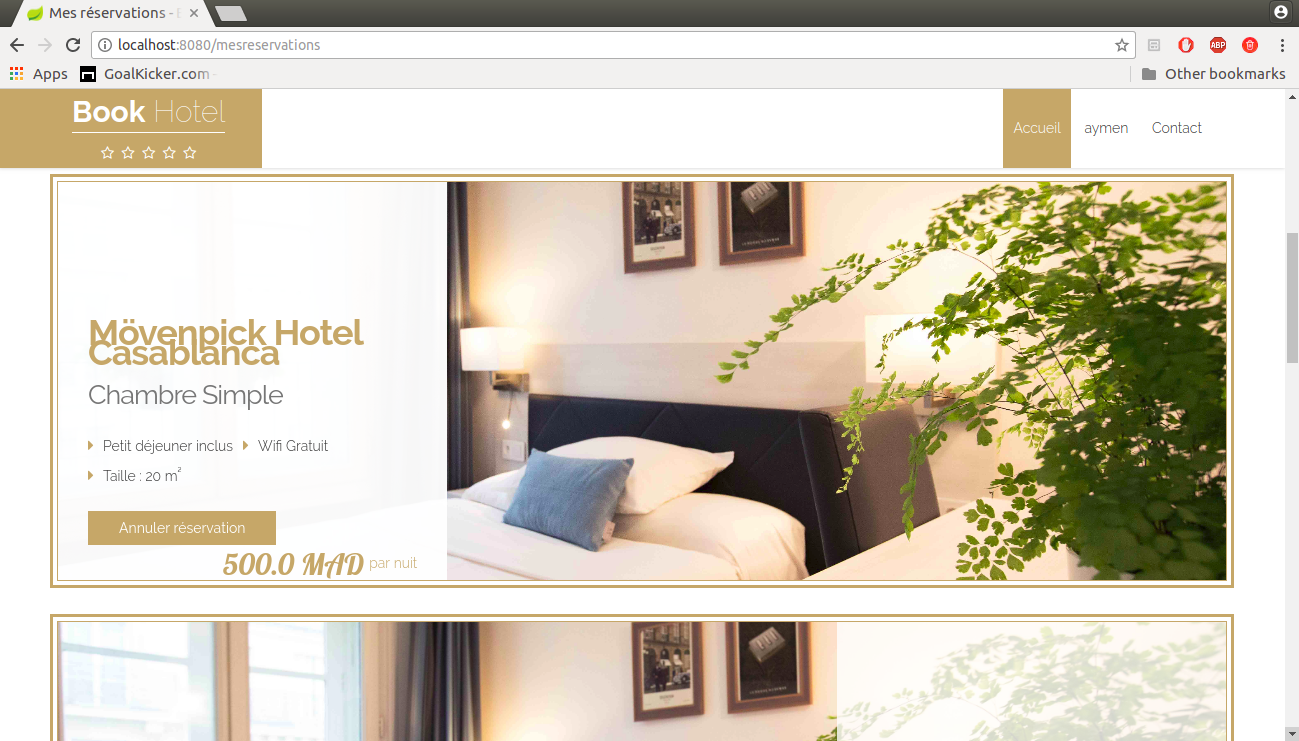
\includegraphics[scale=0.3]{./graphics/mesreservations.png}
		\caption{Mes réservations}
		\end{figure}
		\newpage		
	
	 
	\section{Partie gérant}
	\subsection{Modification des informations de l'hôtel}
	\begin{figure}[!hbtp]
		\centering
		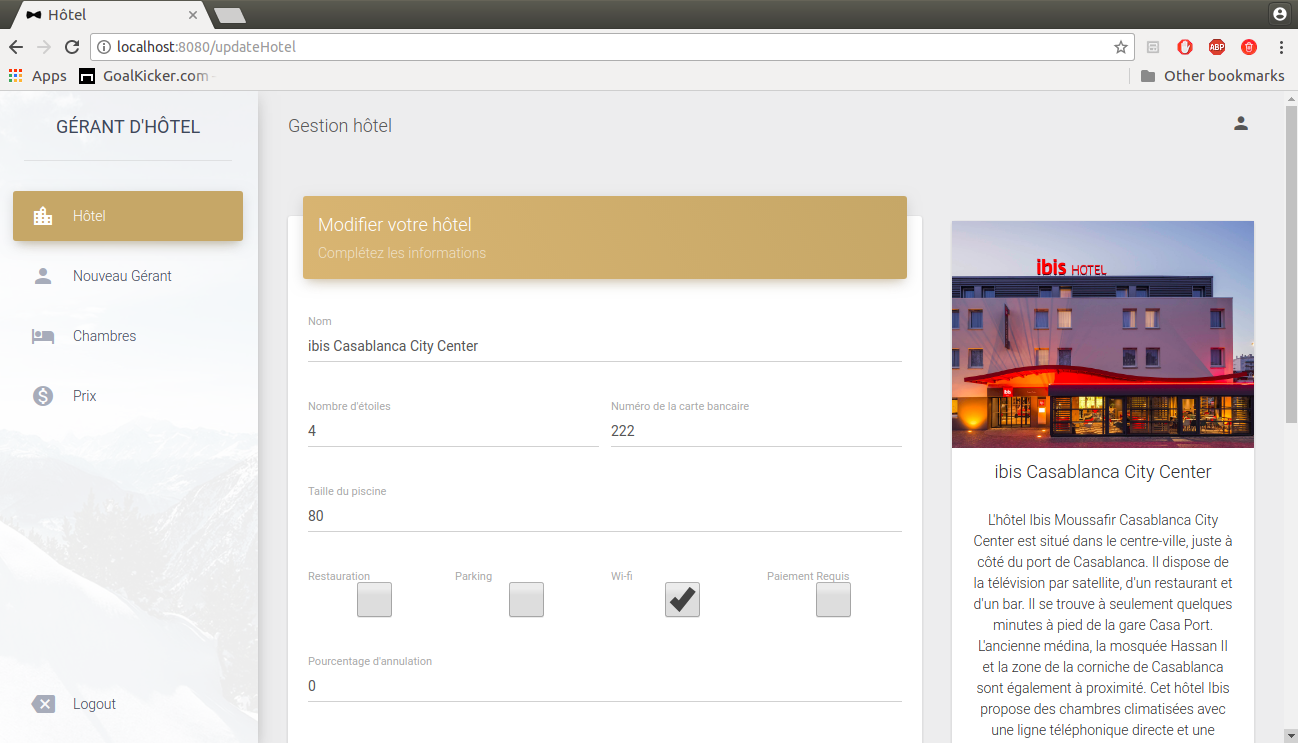
\includegraphics[scale=0.3]{./graphics/updatehotel.png}
		\caption{Modification des informations de l'hôtel}
		\end{figure}
		\newpage	

	\subsection{Ajout d'un gérant}
	\begin{figure}[!hbtp]
		\centering
		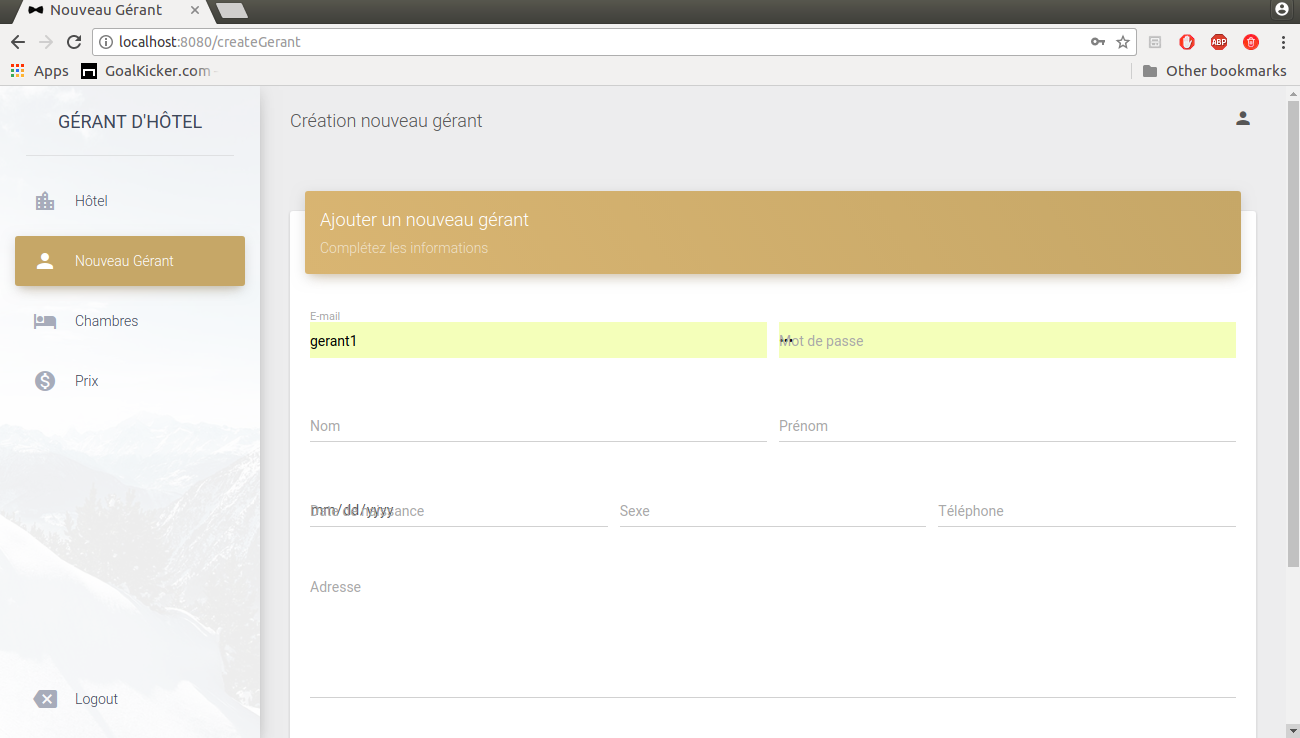
\includegraphics[scale=0.3]{./graphics/nvg.png}
		\caption{Ajout d'un gérant}
		\end{figure}
		\newpage

	\subsection{Gestion des chambres}
Le gérant peut consulter, filtrer,ajouter, modifier, et supprimer les chambres.
	\begin{figure}[!hbtp]
		\centering
		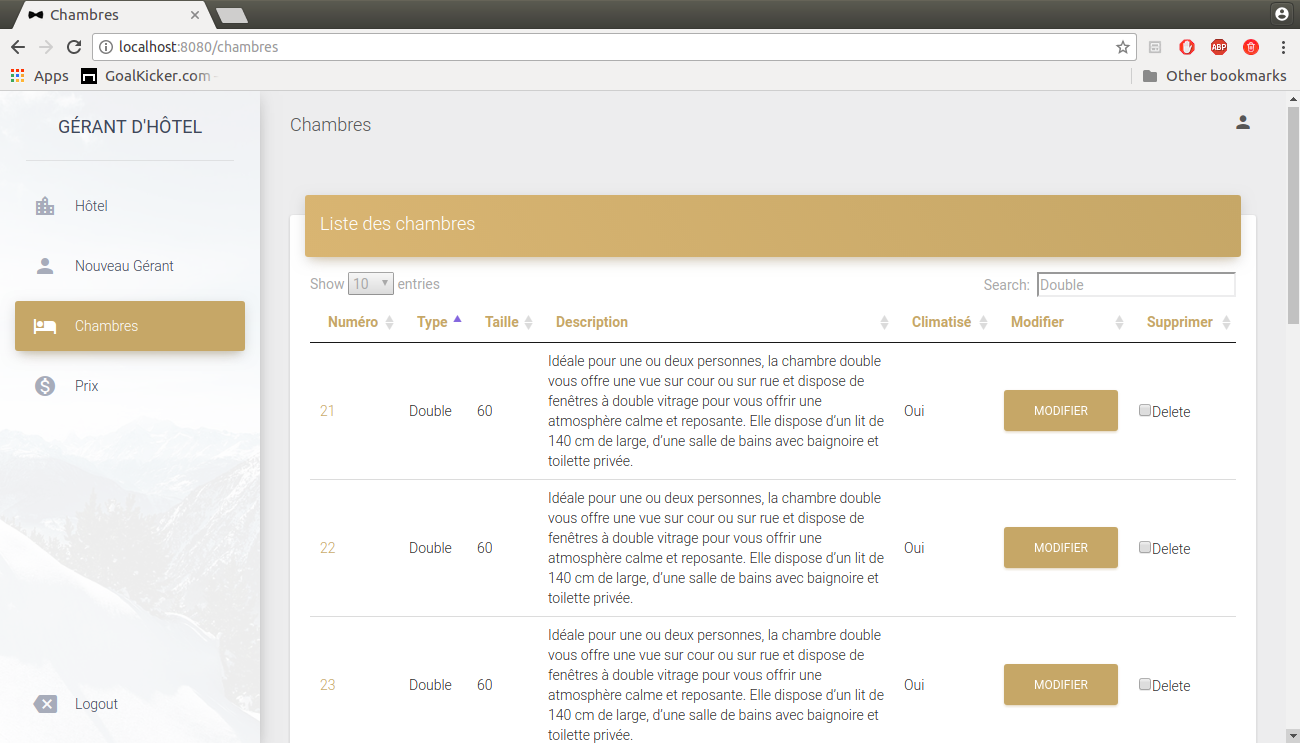
\includegraphics[scale=0.3]{./graphics/chambres.png}
		\caption{Gestion des chambres}
		\end{figure}
		\newpage

	\subsection{Gestion des prix}
Le gérant peut consulter, filtrer, et ajouter des prix selon des périodes.
	\begin{figure}[!hbtp]
		\centering
		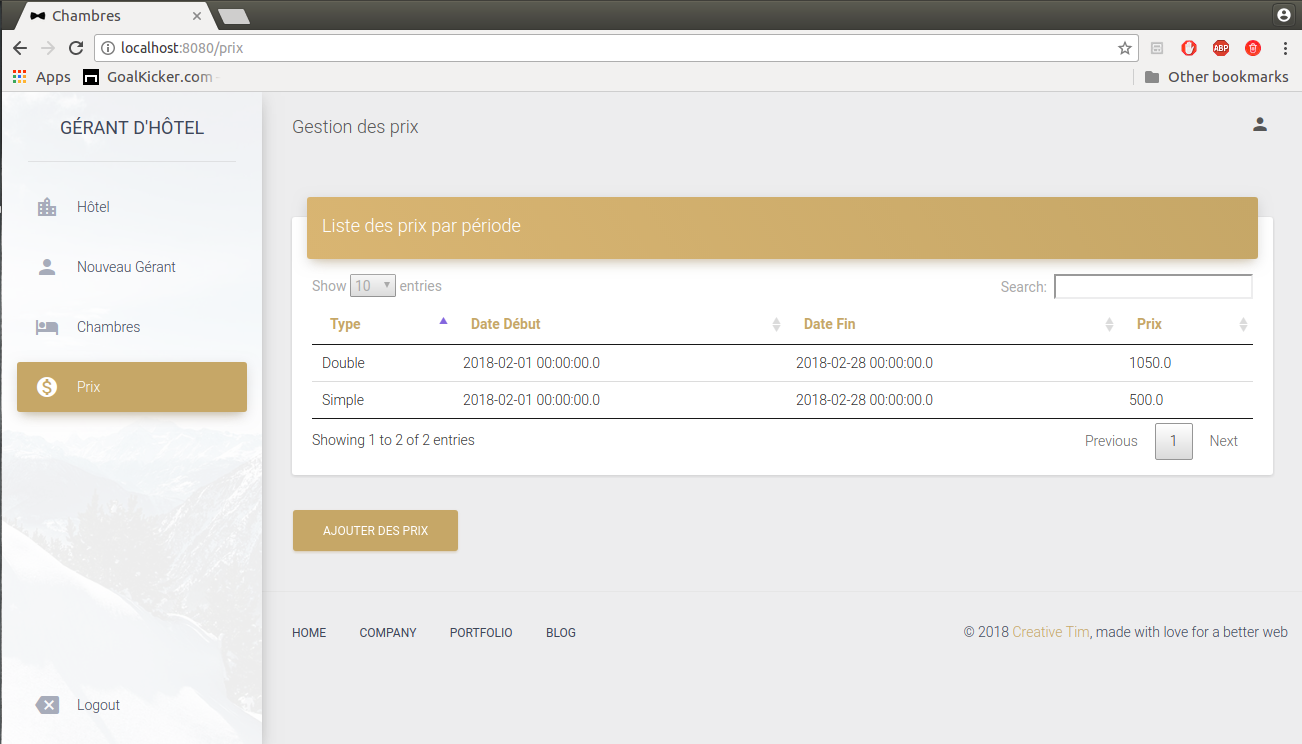
\includegraphics[scale=0.3]{./graphics/prix.png}
		\caption{Gestion des prix}
		\end{figure}
		\newpage

	\section{Partie administrateur}
	\subsection{Gestion des hôtels}
L'admin peut consulter, filtrer,ajouter, et supprimer les chambres.
	\begin{figure}[!hbtp]
		\centering
		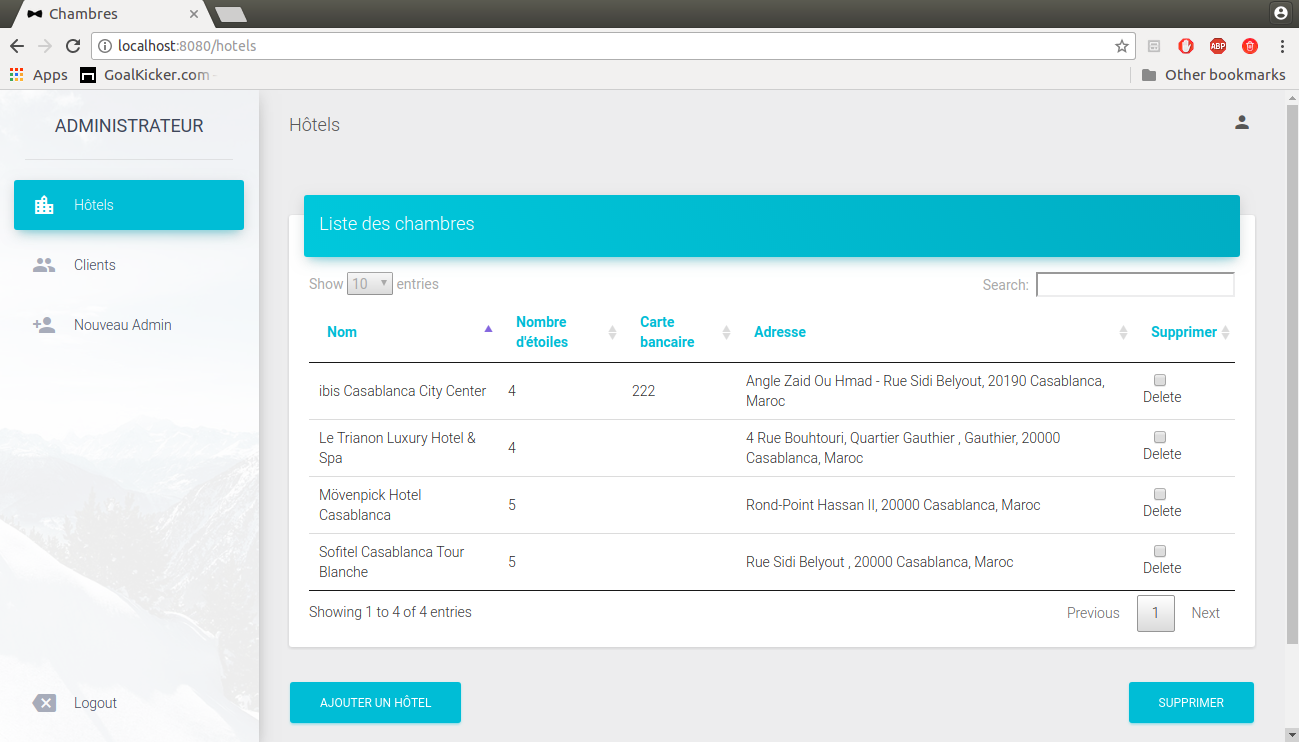
\includegraphics[scale=0.3]{./graphics/hotels.png}
		\caption{Gestion des hôtels}
		\end{figure}
		\newpage

	\subsection{Ajout d'un administrateur}
	\begin{figure}[!hbtp]
		\centering
		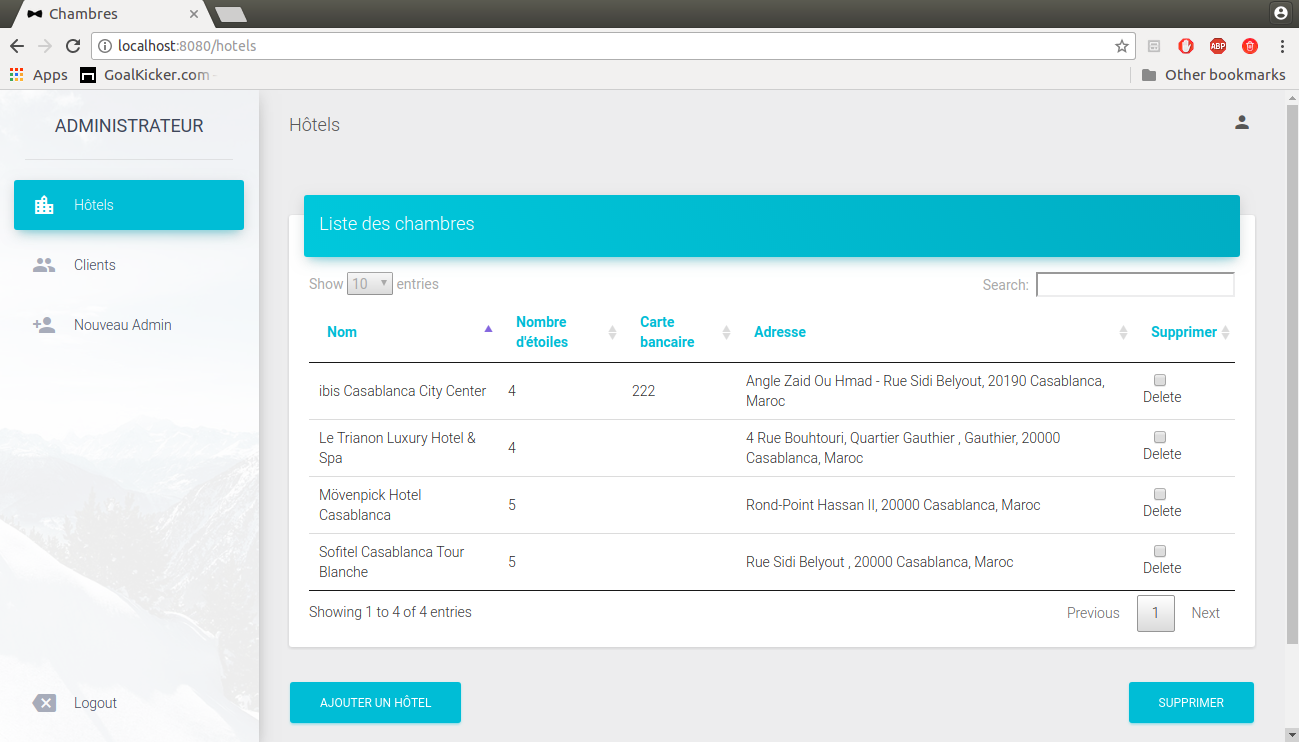
\includegraphics[scale=0.3]{./graphics/hotels.png}
		\caption{Ajout d'un administrateur}
		\end{figure}
		\newpage
	
	\section{Conclusion}
Au cours de ce chapitre, nous avons présenté la dernière étape du développement, qui est
celle de la réalisation et de la mise en œuvre du projet. Nous avons présenté le résultat de la fusion
de tous les éléments de spécifications fonctionnelles et techniques précédemment traitées.
%====================================fin réalisation=================================




%=================================conclusion générale==========================

		\chapter*{Conclusion générale} 
	\addcontentsline{toc}{chapter}{Conclusion}
	Ce projet avait pour but majeur la solidification et la mise en
pratique de l’ensemble des compétences théoriques et techniques acquises durant le premier semestre de la deuxième année filière IWIM. Il
consistait à travailler sur une application web pour automatiser le processus de réservations d'hôtels pour donner au client un service confortable.\\
Malgré la limite du temps réservé à la réalisation de ce projet qui demeure pour nous un projet
de taille et complexité assez importantes et les difficultées que nous avons rencontrés lors de la phase de réalisation que ça soit les bugs, les problèmes de configuration, nous avons pu concrétiser les objectifs tracés initialement, dans les délais estimés. Au début,nous avons commencé par la rédaction du cahier des charges nous avons passé aux
spécifications techniques et fonctionnelles. Après validation de ces spécifications, nous nous sommes mis à développer l'application.\\
Effectivement l'application n'est pas parfaite et beaucoup de choses peuvent être ajoutées ou bien modifiées.\\
En matière de ce projet, nous avons eu l’opportunité d’acquérir de nouveaux concepts, dont les principaux sont le développement d'applications web avec les frameworks Spring et Hibernate, ce qui est vraiment intéressant pour les prochains projets.\\
	
	\chapter*{Webographie}
	\addcontentsline{toc}{chapter}{Webographie}
	\bibliographystyle{plain}
	\vspace{2cm}
	  \begin{itemize}

			\item https://docs.spring.io/spring/docs/current/spring-framework-reference/web.html
			\item http://hibernate.org/orm/documentation/5.2/
			\item https://docs.spring.io/spring-data/jpa/docs/current/reference/html/
			\item https://stackoverflow.com
		\end{itemize}
	\end{document}
\end{document}
